% ICE: Infinite Context Engine — TMLR submission (anonymized, double-blind).
% Generated from ICE_paper.tex by swapping the generic preamble for the official
% TMLR style (tmlr.sty / tmlr.bst from github.com/JmlrOrg/tmlr-style-file).
%
% SUBMISSION (this file, default): authors are auto-hidden by tmlr.sty ->
%   header reads "Under review as submission to TMLR", byline "Anonymous authors".
% CAMERA-READY (after acceptance): change the line below to
%   \usepackage[accepted]{tmlr}, set \month/\year/\openreview, and uncomment the
%   real \author block. For a de-anonymized preprint (e.g. arXiv), use
%   \usepackage[preprint]{tmlr} instead.
\documentclass[10pt]{article}

\usepackage{tmlr}

% --- Packages carried over from the generic version (unchanged) ---
\usepackage{booktabs}
\usepackage{multirow}
\usepackage{amsmath}
\usepackage{amssymb}
\usepackage{graphicx}
\usepackage{xcolor}
\usepackage{enumitem}
\usepackage{microtype}
\usepackage{url}
\usepackage[htt]{hyphenat} % allow hyphenation of \texttt{} content (long code identifiers)
\sloppy
\tolerance=2000
\emergencystretch=3em
% natbib is loaded by tmlr.sty (authoryear, round) — do NOT reload it here.
\usepackage[colorlinks=true,linkcolor=blue!50!black,citecolor=blue!50!black,urlcolor=blue!50!black]{hyperref}
\usepackage{cleveref}
\usepackage{caption}
\usepackage{array}
\usepackage{ragged2e}
\usepackage{pgfplots}
\pgfplotsset{compat=1.18}
\usetikzlibrary{patterns,arrows.meta,positioning,fit,backgrounds,calc}

% --- Shared styles for the architecture diagrams ---
\tikzset{
  icebox/.style={draw=blue!40!black, fill=blue!5, rounded corners=2pt,
    align=center, font=\scriptsize, inner sep=3pt, minimum height=6mm},
  icephase/.style={draw=gray!50, fill=gray!8, rounded corners=3pt,
    align=center, font=\scriptsize\bfseries, inner sep=4pt},
  icestore/.style={draw=teal!50!black, fill=teal!8, rounded corners=2pt,
    align=center, font=\scriptsize, inner sep=3pt, minimum width=17mm, minimum height=9mm},
  iceleg/.style={draw=orange!60!black, fill=orange!8, rounded corners=2pt,
    align=center, font=\scriptsize, inner sep=2pt, minimum width=15mm, minimum height=6mm},
  icecore/.style={draw=red!50!black, fill=red!6, rounded corners=2pt,
    align=center, font=\scriptsize\bfseries, inner sep=3pt},
  iceflow/.style={-{Stealth[length=2mm]}, draw=gray!60, thick},
  iceflowd/.style={-{Stealth[length=2mm]}, draw=gray!60, thick, dashed},
}

% --- Table helpers ---
\newcolumntype{L}[1]{>{\raggedright\arraybackslash}p{#1}}
\newcolumntype{C}[1]{>{\centering\arraybackslash}p{#1}}
\newcolumntype{R}[1]{>{\raggedleft\arraybackslash}p{#1}}

% --- Float placement tuning (kept from the generic version) ---
\setlength{\textfloatsep}{10pt plus 2pt minus 2pt}
\setlength{\intextsep}{8pt plus 2pt minus 2pt}
\renewcommand{\floatpagefraction}{0.7}
\setcounter{topnumber}{3}
\setcounter{bottomnumber}{2}
\setcounter{totalnumber}{5}
\renewcommand{\arraystretch}{1.15}
\captionsetup{font=small,labelfont=bf}

% --- Camera-ready metadata (used only with [accepted]; ignored in submission) ---
\def\month{MM}
\def\year{YYYY}
\def\openreview{\url{https://openreview.net/forum?id=XXXX}}

\title{Curation Over Collection: A Local-First Conversational Memory System and a Longitudinal Protocol for Evaluating It}

% Anonymized for double-blind submission. The tmlr package hides this and prints
% "Anonymous authors" automatically; it is kept anonymous here so no name leaks
% into the PDF. For the camera-ready ([accepted]) version, replace with:
%   \author{\name Deepesh Sonar \email 18deepnar@gmail.com \\
%           \addr Thakur College of Engineering and Technology,\\
%           Computer Engineering, Mumbai, India}
\author{\name Anonymous Author(s) \\ \addr Anonymized for double-blind review}

\begin{document}

\maketitle

\begin{abstract}
Conversational assistants forget everything between sessions, forcing users to re-establish context continually. We present a local-first, multi-store memory system that sits between the user and any OpenAI-compatible model, maintaining persistent memory across arbitrarily long histories through episodic, knowledge-graph, procedural, and document stores with fused, decay-weighted retrieval under a per-query token budget. To evaluate such systems---where static benchmarks cannot capture memory that accumulates, decays, and is revised over months---we introduce LSREP, a Longitudinal State-Replay Evaluation Protocol that replays real, self-authored conversations (1{,}985 turns; 1{,}211 probes across 50 checkpoints) through the system, reconstructing full memory state at each checkpoint and scoring answers against an evolving ground truth. On answer quality the system ties a strong vector-RAG baseline (paired $\Delta = +0.00$, 95\% CI $[-0.07, +0.07]$) while injecting 32\% fewer fragments and winning a materially higher share of blind head-to-head comparisons (30.6\% vs.\ 21.2\%, non-overlapping CIs); under extreme per-turn context density the unbudgeted baseline collapses (94.2\% failure) while the budgeted system holds (mean 4.33). A cumulative ablation shows that adding an unfused lexical signal is harmful ($-0.74$, $[-1.14, -0.36]$) and that rank fusion is corrective ($+0.82$, $[+0.39, +1.24]$). Notably, these gains were obtained with several of the more ambitious stores (knowledge-graph, procedural, and document memory) immature or inactive at the evaluated snapshot---so the result is carried by curation, fusion, and the token budget alone, which if anything sharpens the central principle: memory is curation, not collection. We release the system and the protocol, and report this evaluation candidly as a first honest measurement rather than a finished verdict.
\end{abstract}

%======================================================================
\section{Introduction}

A language model holds a conversation only for as long as its context window holds the conversation; everything older is silently gone, and the interface gives no warning that it happened. We call the resulting failure \emph{context collapse}. Its clearest form, for us, occurs during creative or narrative work and in long technical discussions. The model usually retains the general idea of what is going on, but forgets specificity: the exact rule that was set, a particular character, a precise decision made yesterday, the FastAPI dependency-injection pattern established three months ago. The conversation continues, but the model has quietly lost the thread. Worse, the workarounds---exporting chats, copying and pasting into a fresh context, and re-explaining everything for the third time---work for the first few exchanges of a new session and then degrade, because the AI that started coherent is, by turn fifteen, a different AI that has lost the new context too. Every conversational AI interface in existence today suffers from the same fundamental flaw: amnesia. Each new session begins with complete cognitive silence.

This is not a minor inconvenience. For a human doing serious work---building a complex software system over months, constructing an original fictional universe across hundreds of sessions, planning a multi-year academic trajectory---the lack of persistent, intelligent, user-controlled memory is the single largest bottleneck between the human and the AI working as genuine collaborators. The systems designed to address this---CLAUDE.md, \texttt{.cursorrules}, the memory layers in cloud APIs---either cap at a few hundred lines, go stale, or exist in someone else's cloud with no user control over what is remembered and what is forgotten.

The Infinite Context Engine (ICE) is a local-first, personal AI memory middleware for human-AI conversational interfaces. It sits between the user and their language models---classifying every prompt, deciding which memories to surface, routing to the right model, managing the accumulation of knowledge over time, and injecting precisely the right context into every LLM call. ICE is not a coding agent. It is not a background tool that watches a developer's file system. It is infrastructure for the thinking layer---for the deep collaborative sessions where the AI needs to remember that two entities are the same entity across different eras, that the user's PostgreSQL schema is partitioned a specific way, or that the user made a particular architectural decision last Tuesday and has already ruled out the alternatives. It is memory for the human mind, not memory for a code compiler.

A crucial architectural assumption underlying ICE is that the language model itself should be treated as a stateless reasoning engine. The model has no memory of past interactions, nor does it need to. ICE does not attempt to embed memory into the model's weights through fine-tuning or continual learning; instead, it externalises memory entirely, storing, maintaining, and retrieving context as an independent system that surrounds the model. The model processes whatever context ICE supplies and forgets it immediately after generation. This separation is deliberate: it allows models to be swapped, upgraded, or replaced without losing memory, and it makes the memory system transparent, inspectable, and user-controllable. The vector-RAG baseline shares the superficial property of feeding external context to a stateless model, but it is not \emph{designed} to reconstruct a structured, evolving cognitive state: it stores raw chunks, with no knowledge graph, behavioural-pattern inference, or decay-and-reinforcement lifecycle. ICE is built around exactly those mechanisms---though we report candidly (Section~\ref{sec:limitations}) which of them were actually active at the evaluation snapshot, since the results here rest on its curation and fusion more than on the full cognitive apparatus.

In this paper we make three contributions:

\begin{enumerate}[leftmargin=*]
  \item \textbf{A local-first conversational memory system} (ICE)---a multi-store architecture (episodic, a temporally-versioned knowledge graph, procedural, and document memory) with intent-driven retrieval routing, access-weighted decay, and a dynamic per-query token budget, released in full.
  \item \textbf{LSREP} (Longitudinal State-Replay Evaluation Protocol)---a benchmark, motivated by the failure of static precision-based metrics, that replays months of real conversational history through the system, reconstructs full memory state at each of many temporal checkpoints, and scores answers against an \emph{evolving} ground truth. This is the paper's most reusable contribution, and it is independent of any particular memory system.
  \item \textbf{An honest longitudinal evaluation.} The system matches a strong vector-RAG baseline on answer quality while injecting 32\% fewer fragments and winning a substantially larger share of blind head-to-head comparisons; under a context-overflow stress test where the unbudgeted baseline collapses (94.2\% failure) the budgeted system holds (4.33); and a cumulative ablation shows that adding an unfused lexical signal is harmful while rank fusion is corrective. We report candidly that these gains are carried by curation, fusion, and the token budget---several of the more ambitious stores were immature or inactive at the evaluated snapshot (Section~\ref{sec:limitations})---so this is a first honest measurement, not a finished verdict.
\end{enumerate}

The paper is organised as a journey of discovery rather than a victory lap. The evaluation pipeline that we eventually called LSREP was itself born from failure: an earlier precision-based metric could not capture the fact that a retrieved fragment can be ``irrelevant'' at turn 100 yet become critical at turn 800. Section~\ref{sec:exp-design} tells that story. The first full evaluation (Experiment~1) then revealed that the immature system, honestly measured, was worse than the vector baseline on every metric---a sobering result that drove the design of the mature system. The mature system, presented in Experiment~2 and the ablation, is what this paper is actually about.

%======================================================================
\section{Related Work}
\label{sec:related-work}

We organise prior work into four areas, each of which has shaped our design decisions, and we are deliberately critical of the gaps that ICE attempts to address.

\subsection{Stateful Memory and Retrieval-Augmented Architectures}

The architectural constraint of bounded context lengths in transformer-based models has driven the engineering of specialised memory hierarchies designed to preserve user-specific facts over extended temporal horizons. \textbf{MemGPT} \citep{packer2023memgpt} conceptualises the LLM context window as a form of primary random-access memory, backed by an unbounded external storage system, employing an intelligent paging mechanism to manage the control flow of data between the main context and external tiers, effectively creating the illusion of an infinite context window. While MemGPT demonstrates high efficacy in short-to-medium length interactions and intensive document analysis tasks, empirical stress tests reveal significant degradation in highly extended, multi-session dialogues. The system relies heavily on flat, dense vector retrieval, which struggles with the ``compaction continuity problem'' and fails to distinguish between semantically identical but contextually distinct entities over time. Crucially, MemGPT lacks a structured knowledge graph to track the temporal evolution of entities and operates without intent-driven retrieval routing, leading to context dilution in complex narrative environments.

To address the latency and token-cost bottlenecks associated with hierarchical paging, \textbf{mem0} \citep{chhikara2025mem0} proposed a lightweight, production-ready memory layer that optimises the memory lifecycle by employing a single-pass, append-only extraction pipeline that distils long-form conversations into atomic, non-hierarchical facts. By utilising a multi-signal retrieval pipeline that fuses semantic embedding, BM25 keyword matching, and entity linking in parallel, mem0 achieves significant reductions in computational overhead, excelling on benchmarks such as LoCoMo and LongMemEval. Despite its efficiency, the reliance on topologically flat, key-value fact extraction inherently limits the system's cognitive depth. It lacks the capacity for versioned entities, meaning contradictory or evolving facts are not systematically reconciled, and it does not natively support procedural memory or implement a mathematically grounded decay and archival mechanism.

\textbf{MemoryBank} \citep{zhong2024memorybank} advanced the cognitive plausibility of long-term agentic memory with an architecture heavily inspired by human psychology. MemoryBank integrates the Ebbinghaus Forgetting Curve to model memory updates via a time-aware decay and reinforcement mechanism, where every memory item maintains a continuously updated strength score. Applied to the SiliconFriend conversational agent, MemoryBank successfully maintains persona invariance and heightened empathy in multi-day dialogues. However, the system is fundamentally constrained by its retrieval substrate: it lacks a foundational knowledge graph to facilitate associative, multi-hop reasoning, and it fails to implement conversation-scoped clustering, which is essential for maintaining narrative coherence across disparate conversational threads.

\textbf{SCMoE} \citep{shi2024scmoe} developed the Self-Contrast Mixture-of-Experts framework to address the computational bottlenecks of dense memory retrieval. SCMoE introduces a training-free strategy that utilises unchosen experts in a self-contrast manner during inference, determining next-token probabilities by contrasting the output logits from strong and weak activations. While SCMoE optimises the internal routing of neural representations for better information processing, its application as an externalised memory retrieval system remains undertested, and it has not been stress-tested on the large, dynamically shifting per-turn documents that characterise persistent agentic memory.

The structural vulnerabilities of these systems underscore a pervasive industry trend: the conflation of static fact-storage with dynamic working memory. ICE addresses these precise vulnerabilities by bridging the gap between efficient retrieval and temporal narrative continuity.

\subsection{Knowledge Graphs as Dialogue Substrates}

To overcome the relational blindness of topologically flat vector stores, the literature has increasingly explored knowledge graphs (KGs) to map the intricate semantic topologies of textual data. \textbf{GraphRAG} \citep{edge2024graphrag} introduced a method designed to answer global, sense-making queries over extensive, private document collections. Traditional vector-based retrieval fails on query-focused summarisation tasks that require traversing an entire corpus. GraphRAG circumvents this by utilising an LLM to extract a massive entity knowledge graph from raw text, followed by the application of community detection algorithms (e.g., Leiden) to partition the graph. It then pre-generates hierarchical community summaries for groups of closely related entities. While GraphRAG significantly improves answer depth, it operates under the assumption of a temporally static corpus. In GraphRAG, all ingested facts are treated as equally current; it lacks the temporal versioning required to track an entity whose properties, relationships, or states mutate dynamically across multiple conversational sessions.

\textbf{KGP} \citep{wang2023kgp} proposed Knowledge Graph Prompting to address the specific challenges of multi-document question answering. KGP constructs a specialised graph where nodes represent individual passages or document structures, and edges denote semantic or lexical similarities. The framework deploys an LLM-based graph traversal agent that acts as a local navigator, dynamically gathering supporting context to regulate the transitional space among interconnected documents. Concurrently, \textbf{Think-on-Graph (ToG)} \citep{sun2024tog} developed a tight-coupling algorithmic framework that treats the LLM as an active agent performing iterative beam search across KG paths, prompting the LLM to explore multiple possible reasoning paths dynamically and pruning irrelevant branches until it determines that a question can be answered.

While both KGP and ToG demonstrate the profound utility of structural graph retrieval, their architectures are heavily tailored for single-shot, objective question answering over static knowledge bases. They inherently assume the graph is a ground-truth repository of factual world knowledge, completely missing the mechanisms for narrative continuity, belief decay, and contradiction resolution required for an evolving conversational agent. ICE leverages the topological benefits of these graph systems but repurposes them to support a continuously mutating conversational landscape.

\subsection{Evolutions in Classic Retrieval-Augmented Generation}

The foundational models of retrieval-augmented generation established the paradigm of augmenting parametric model knowledge with non-parametric, external databases to mitigate hallucinations. \textbf{RAG} \citep{lewis2020rag} formalised the original framework, providing a general-purpose fine-tuning recipe that combines a pre-trained sequence-to-sequence model with a dense vector index of a static document corpus, such as Wikipedia. While this fundamentally shifted how models access long-tailed knowledge, classic RAG relies on point-in-time document retrieval driven by maximum inner product search. Conversational history, by contrast, is not a static corpus. It grows organically, facts are frequently updated or contradicted, and context shifts dynamically. The original RAG architecture possesses no mechanisms to handle these temporal dynamics.

Subsequent iterations sought to optimise the retrieval, encoding, and decoding pipelines. \textbf{REALM} \citep{guu2020realm} integrated a latent knowledge retriever directly into the unsupervised pre-training phase, while \textbf{Fusion-in-Decoder (FiD)} \citep{izacard2021fid} processes retrieved passages independently in the encoder before concatenating them for joint attention in the decoder, allowing the model to dynamically weigh and aggregate evidence from up to a hundred retrieved passages. \textbf{REPLUG} \citep{shi2024replug} treats the generative LLM as an entirely frozen black box, optimising the retrieval model using perplexity scoring signals. \textbf{CRAG} \citep{yan2024crag} applies an explicit corrective process to mitigate retrieval noise, implementing a lightweight evaluator that scores retrieved documents and triggers a decompose-then-recompose algorithm to filter irrelevant spans.

Despite their mathematical and architectural elegance, REALM, FiD, REPLUG, and CRAG are structurally confined to static knowledge bases. They possess no innate mechanisms to handle a personalised, highly dynamic, and evolving conversation history where a user's preferences, constraints, and state of mind shift iteratively. ICE replaces the static-corpus assumption with a highly mutable, chronologically aware middleware designed specifically for personal agentic history.

\subsection{Algorithmic Primitives in ICE}

To achieve resilient memory retrieval, ICE synthesises several foundational algorithmic techniques. \textbf{BM25} \citep{robertson2009bm25} remains one of the most successful sparse retrieval algorithms, scoring document relevance based on a non-linear term frequency function and inverse document frequency, with document length normalisation. While dense semantic embeddings excel at capturing conceptual similarity, they frequently suffer from catastrophic failures in exact-keyword matching. BM25 ensures high-fidelity lexical recall and serves as a secondary leg in ICE's multi-signal retrieval strategy. \textbf{Reciprocal Rank Fusion} \citep{cormack2009rrf} is the mathematically elegant algorithm that combines document rankings by sorting them based on the inverse of their rank positions across multiple independent search systems, preventing any single retrieval methodology from disproportionately skewing the results. RRF is ICE's fusion backbone, and our ablation finds it \emph{corrective}: it rescues a multi-signal retriever from the noise that an unfused lexical leg injects (Section~\ref{sec:ablation}), rather than lifting quality above a strong single-leg baseline. \textbf{HyDE} \citep{gao2023hyde} addresses the vocabulary-mismatch problem by generating a hypothetical document from the query and embedding that instead; ICE implements it as an optional gated rewrite, but we note up front that it was disabled in our evaluation build, so we make no empirical claim about it here.

\subsection{The Gap}

The gap in prior work is not any single missing feature---it is the combination of temporal awareness, structured entity memory, intent-driven retrieval routing, and a per-query token budget. Systems that add one of these still fail on the specific use case that motivated ICE: a long-running creative or technical project in which entities evolve, intentions shift, and conversation history must be filtered as much as retrieved.

%======================================================================
\section{Datasets}
\label{sec:datasets}

The evaluation uses four long-form conversational datasets, all authored by a single user over periods ranging from months to years. We use anonymised descriptive labels rather than the internal names. \cref{tab:datasets} summarises them.

\begin{table}[htbp]
\centering
\small
\caption{Four evaluation datasets (anonymised). All are single-user, self-authored. The ``Stress dimension'' column indicates which aspect of the ICE architecture each dataset most heavily exercises.}
\label{tab:datasets}
\begin{tabular}{@{}L{3.1cm}L{3.6cm}rrL{3.2cm}@{}}
\toprule
\textbf{Label} & \textbf{Description} & \textbf{Turns} & \textbf{Ckpts.} & \textbf{Stress dimension} \\
\midrule
Dataset A (Creative Writing) & Collaborative fan-fiction writing session & 290   & 10 & Narrative continuity, character evolution \\
Dataset B (Long-Form Creative) & Fantasy world-building and story-planning & 1{,}119 & 20 & Temporal-horizon retrieval, entity evolution \\
Dataset C (Technical Planning) & Design and development of ICE itself       & 325   & 8  & Information density, 8K+ token turns \\
Dataset D (Academic Planning) & Graduate school and career planning       & 251   & 12 & Mixed personal/technical, decision tracking \\
\midrule
\textbf{Total} & & \textbf{1{,}985} & \textbf{50} & \\
\bottomrule
\end{tabular}
\end{table}

Each dataset was selected for three reasons. First, all four are substantially longer than typical chat interactions (251--1{,}119 turns), providing opportunities for information to become separated by hundreds of turns and creating realistic long-term retrieval challenges. Second, each represents a distinct memory domain---creative-writing datasets emphasise narrative continuity and entity consistency, the technical-planning conversation emphasises design decisions and implementation rationale, and the academic-planning conversation requires tracking personal preferences, goals, and decision histories. Third, all four contain dense memory structures---recurring entities, evolving relationships, technical terminology, procedural patterns, and long-term dependencies---suitable for exercising ICE's multi-retrieval architecture.

We acknowledge the single-user limitation: these conversations are genuinely long and genuinely demanding in ways that synthetic benchmarks are not, but they do not yet represent a diverse population of users.

%======================================================================
\section{System Architecture}
\label{sec:architecture}

ICE is an OpenAI-compatible memory middleware that sits between a conversational client and a pool of locally-served large language models (Ollama / SGLang). It is not a model itself: every request addressed to the synthetic model name \texttt{ice-proxy} is intercepted by a FastAPI proxy that classifies the turn, retrieves relevant context from four long-lived memory stores, assembles a KV-cache-friendly prompt, routes the request to a per-turn specialist model, streams the response back over Server-Sent Events (SSE), and then dispatches a fan-out of background workers that extract, decay, cluster, and crystallise the new turn into long-term memory. The net effect is that any downstream model operates against an effectively unbounded, personalised context that is selectively rebuilt on every turn.

\begin{figure}[t]
\centering
\resizebox{0.92\columnwidth}{!}{%
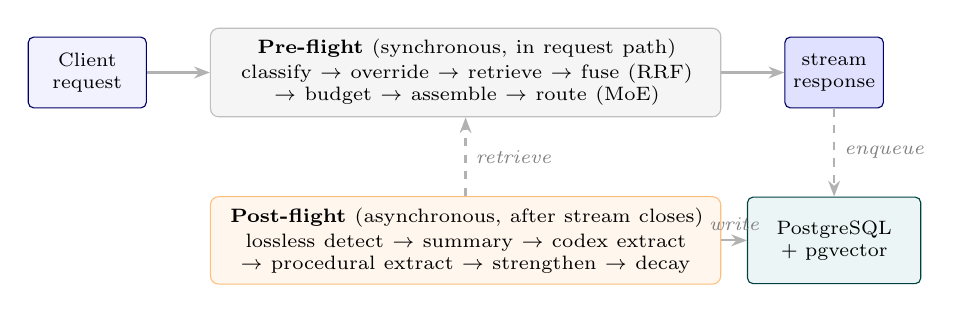
\begin{tikzpicture}[node distance=5mm]
% Client
\node[icebox, minimum width=15mm, minimum height=9mm] (client) {Client\\request};
% Pre-flight phase (single wide box listing the stages)
\node[icephase, right=8mm of client, minimum height=11mm, text width=62mm] (pre)
  {Pre-flight \textnormal{(synchronous, in request path)}\\[1pt]
   \textnormal{\scriptsize classify $\to$ override $\to$ retrieve $\to$ fuse (RRF)}\\
   \textnormal{\scriptsize $\to$ budget $\to$ assemble $\to$ route (MoE)}};
% Stream response
\node[icebox, fill=blue!12, right=8mm of pre, minimum height=9mm] (stream) {stream\\response};
% Post-flight phase (below pre-flight)
\node[icephase, fill=orange!7, draw=orange!50, below=10mm of pre, minimum height=11mm, text width=62mm] (post)
  {Post-flight \textnormal{(asynchronous, after stream closes)}\\[1pt]
   \textnormal{\scriptsize lossless detect $\to$ summary $\to$ codex extract}\\
   \textnormal{\scriptsize $\to$ procedural extract $\to$ strengthen $\to$ decay}};
% Datastore, to the right of post-flight, aligned under stream
\node[icestore, minimum width=22mm, minimum height=11mm] (db) at (stream |- post) {PostgreSQL\\+ pgvector};
% --- Arrows ---
\draw[iceflow] (client) -- (pre);                       % request in
\draw[iceflow] (pre) -- (stream);                       % stream out
\draw[iceflowd] (stream) -- (db) node[midway, right, font=\scriptsize\itshape, gray] {enqueue};  % async handoff
\draw[iceflow] (post) -- (db) node[midway, above, font=\scriptsize\itshape, gray] {write};        % post-flight writes
\draw[iceflowd] (post.north) -- (pre.south) node[midway, right, font=\scriptsize\itshape, gray] {retrieve}; % feeds next retrieval
\end{tikzpicture}%
}
\caption{ICE system overview. The pre-flight phase runs synchronously in the request path; the post-flight phase runs asynchronously after the stream closes.}
\label{fig:system-overview}
\end{figure}

Each turn traverses a \textbf{pre-flight} (synchronous, in the request path) and a \textbf{post-flight} (asynchronous, after the stream closes) phase. In the pre-flight phase the user message is classified by a two-stage pipeline---a rule-based Dynamic Intent Inferencer (DI3) followed, on miss, by a 25-way PyTorch MLP---producing topic tags, intent tags, and a context-reliance label. Hard override rules then coerce the label (e.g.\ Creative\_\&\_Media $\Rightarrow$ Long\_Term\_Memory). A Hybrid Retrieval Orchestrator runs six retrieval legs (BM25, vector with decay weighting, Codex graph traversal, procedural, RAG, batch summaries)\footnote{Six by \emph{design}. At the evaluated snapshot only the two episodic legs (BM25, vector) plus a small Codex contribution were live; the procedural, RAG, and batch-summary legs returned nothing (a pgvector-binding bug in two, an empty store in the third). The reported results therefore reflect an effectively three-source system---see Section~\ref{sec:limitations}.}, fuses them with weighted Reciprocal Rank Fusion (RRF), and post-processes the fused list with bonuses, session diversification, deduplication, and a dynamic token budget. A Prompt Assembler concatenates the retrieved fragments with persistent memory slots, recent turns, and the live user message under a stable prefix that maximises KV-cache reuse. Finally, a Mixture-of-Experts (MoE) router selects the best locally-served model for the assembled prompt, with per-conversation stickiness. In the post-flight phase a Post-Flight Evaluator runs lossless detection and summary generation, unconditionally dispatches a Procedural Extractor and, conditionally on the lossless flag, a Codex Extractor; both are idempotent Celery tasks. A fan-out of scheduled background workers---decay, clustering, reflection, batch summariser, sentinel monitor, and a weekly fine-tune worker---maintains the memory stores over time.

\subsection{Classification Engine}

The classification engine produces, for each user turn, a triple of outputs: a set of topic tags, a set of intent tags, and a single context-reliance label. These three outputs drive every downstream decision---which retrieval legs are weighted, how the token budget is split, whether the wide-net fallback fires, and which model the MoE router selects. The engine is deliberately a two-stage cascade: a cheap rule-based pre-classifier resolves obvious cases in microseconds, and a small PyTorch MLP resolves everything else with sub-millisecond CPU inference.

The MLP is a deliberately tiny classifier (a 384 $\rightarrow$ 128 $\rightarrow$ 25 multi-layer perceptron with ReLU and 0.3 dropout). The input is a single 384-dimensional embedding produced by a frozen \texttt{Qwen/Qwen3-Embedding-0.6B} embedder; the single shared linear head is sliced at inference time into three blocks: 11 topic labels, 11 intent labels, and 3 context-reliance classes (Zero\_Shot, Long\_Term\_Memory, Real\_Time\_Search). Topic and intent are decoded multi-label (sigmoid, threshold 0.3, argmax fallback); context-reliance is decoded single-label (softmax, argmax).

DI3 (gated by a settings flag) is a rule-based pre-classifier that catches obvious cases before the MLP runs. It computes five density signals in $[0,1]$ from the raw prompt: code density (token-weighted sum over code features), sentiment density (lexicon match), meta density (references to the model itself), noise density (short, alpha-poor, keyboard-mash), and reference density (anaphoric terms like ``this'', ``that'', ``it''). DI3 evaluates five rules in order, returning the first that fires, or none, in which case the MLP runs. The reference rule is special: it returns empty topic and intent tags but forces Long\_Term\_Memory, and the orchestrator then runs the MLP only to obtain the topic and intent labels. A two-tier threshold on the reference rule (0.2 for short conversations, 0.1 once the conversation exceeds ten turns) is the engine's primary mechanism for implementing a long-conversation LTM bias.

\textbf{Override rules.} After DI3 or the MLP produces a result, three rules run in evaluation order: (i)~LTM immutability---once Long\_Term\_Memory is set, no override may downgrade it; (ii)~Creative\_\&\_Media $\Rightarrow$ LTM; (iii)~Software\_\&\_Tech + anaphora $\Rightarrow$ LTM (substring check on 23 referential words including ``my'', ``our'', ``this'', ``previous''). A second, API-level LTM bias lives outside the classifier: when a conversation has more than ten turns or the classifier's max\_confidence $< 0.95$, a Zero\_Shot context-reliance label is upgraded to Long\_Term\_Memory before retrieval runs.

\textbf{Context-aware classification.} When a conversation ID is supplied, the MLP path queries the last three episodic-memory turns for that conversation (n=3, max\_total\_words=500), preferring summary\_text and falling back to the first 150 words of raw\_text. The context is prepended to the prompt as natural-language text before embedding.

\subsection{Memory Architecture}

ICE maintains \textbf{four distinct memory stores}, plus Memory Slots (persistent structured working memory), Context Clusters (conversation-scoped topical clusters), and a cold-storage archive. All stores live in a single PostgreSQL database with the pgvector extension; every vector column is \texttt{Vector(384)} because the same Qwen3-Embedding-0.6B embedder is used everywhere.

\begin{figure}[t]
\centering
\resizebox{0.9\columnwidth}{!}{%
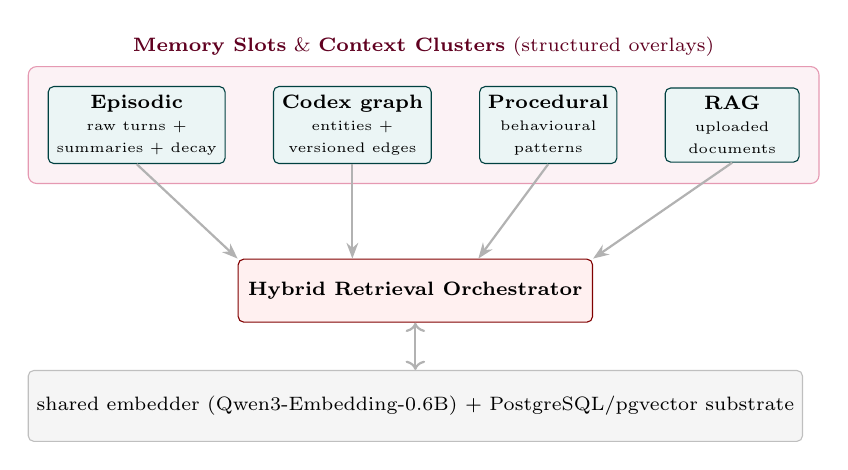
\begin{tikzpicture}[node distance=4mm]
% Four stores
\node[icestore] (epi) {\textbf{Episodic}\\{\tiny raw turns +}\\{\tiny summaries + decay}};
\node[icestore, right=6mm of epi] (codex) {\textbf{Codex graph}\\{\tiny entities +}\\{\tiny versioned edges}};
\node[icestore, right=6mm of codex] (proc) {\textbf{Procedural}\\{\tiny behavioural}\\{\tiny patterns}};
\node[icestore, right=6mm of proc] (rag) {\textbf{RAG}\\{\tiny uploaded}\\{\tiny documents}};
% Overlay layers box behind stores
\begin{scope}[on background layer]
\node[draw=purple!40, fill=purple!5, rounded corners=3pt, fit=(epi)(rag), inner sep=7pt,
  label={[font=\scriptsize, purple!50!black]above:\textbf{Memory Slots} \& \textbf{Context Clusters} (structured overlays)}] (overlay) {};
\end{scope}
% Orchestrator
\node[icecore, below=12mm of codex, xshift=8mm, minimum width=45mm, minimum height=8mm] (orch) {Hybrid Retrieval Orchestrator};
% Shared substrate
\node[icestore, below=6mm of orch, minimum width=45mm, fill=gray!8, draw=gray!50] (sub) {shared embedder (Qwen3-Embedding-0.6B) $+$ PostgreSQL/pgvector substrate};
% Arrows stores -> orchestrator
\draw[iceflow] (epi.south) -- (orch.north west);
\draw[iceflow] (codex.south) -- ([xshift=-8mm]orch.north);
\draw[iceflow] (proc.south) -- ([xshift=8mm]orch.north);
\draw[iceflow] (rag.south) -- (orch.north east);
\draw[iceflow, <->] (orch) -- (sub);
\end{tikzpicture}%
}
\caption{Memory architecture. The four stores differ in cardinality, schema, and retrieval semantics, but share a common embedder and a common PostgreSQL substrate.}
\label{fig:memory-arch}
\end{figure}

\begin{table}[htbp]
\centering
\small
\caption{The four memory stores. Each store is queried by one or more retrieval legs in the hybrid orchestrator.}
\label{tab:stores}
\begin{tabular}{p{0.20\columnwidth}p{0.42\columnwidth}p{0.28\columnwidth}}
\toprule
\textbf{Store} & \textbf{Purpose / Key columns} & \textbf{Retrieval method} \\
\midrule
Episodic & Every conversational turn; raw\_text, summary\_text, lossless\_flag, decay\_score, access\_count, is\_document, embedding & BM25 leg, vector-with-decay leg, session diversification \\
Codex & Temporally-versioned semantic graph; entities (canonical name, aliases, properties JSONB, context\_payload), typed edges with valid\_from / valid\_until, append-only event log, snapshots & Graph traversal (BFS depth 3, valid\_until IS NULL), MERA enumeration fallback \\
Procedural & Recurring behavioural patterns; pattern\_name, trigger\_conditions, reinforcement\_count, confidence\_score, is\_active & Vector top-5 with hard intent gate (Strategic\_Planning, Generation, Open\_Exploration) \\
RAG & Externally-ingested documents; chunked at 512 words, embedded & Vector top-5, triple-gated (LTM AND (Factual\_Retrieval $\lor$ Analysis\_\&\_Summarization) AND reference keyword) \\
\bottomrule
\end{tabular}
\end{table}

\textbf{Memory slots} are prepended verbatim to every prompt. Seven slot names are server-enforced: \texttt{persona}, \texttt{user\_preferences}, \texttt{tool\_guidelines}, \texttt{project\_context}, \texttt{guidance}, \texttt{pending\_items}, \texttt{session\_patterns}. Slots are written through four paths: direct user update, batch initialisation, Reflection-proposed but user-gated updates (high-stakes slots land in the review queue), and Reflection auto-applied updates to \texttt{pending\_items} only.

\textbf{Context clusters} are conversation-scoped topical groupings. The centroid of member turn embeddings (renormalised to unit length after every change) is a \texttt{Vector(384)}; membership is many-to-many through an episodic\_cluster\_links join table. The clustering worker (beat every 30 min) assigns each unassigned turn to the best existing cluster (combined score: embedding similarity + 0.08 per shared entity + tag overlap) or to a new cluster when no candidate clears a 0.6 similarity threshold.

\textbf{Decay mechanics} are access-weighted. Three independent decay workers (all beat-scheduled every 5{,}400~s for 16 cycles/day) apply per-cycle multipliers: 0.95$^{1/16}$ ($\approx$5\%/day) for unaccessed, non-creative turns; 0.98$^{1/16}$ ($\approx$2\%/day) for accessed, non-creative turns; 0.99$^{1/16}$ ($\approx$1\%/day) for any turn tagged Creative\_\&\_Media. A \textbf{creative floor} clamps decay\_score to 0.3 for creative turns regardless of age or access, protecting long-form narrative from being summarised away. Turns whose decay\_score falls below 0.1 are archived; those that subsequently fall below 0.05 are moved to a minimal cold-storage table and physically deleted from episodic memory. Codex edges decay by a similar mechanism (strength multiplied by 0.99$^{1/16}$; demoted from active to pending once strength $<$ 0.3). Procedural patterns are boolean-deactivated after 180 days if they have fewer than three reinforcements.

\textbf{Batch summaries} group decayed-but-not-archived turns into 50-turn batches; a background model produces a 500-token preservation-prompt summary, and the summary is the second life of a turn---retrievable after the original ages into cold storage.

\subsection{Codex Knowledge Graph}

The Codex is a temporally-versioned, controlled-vocabulary knowledge graph spread over four tables: \texttt{codex\_entities} (canonical name, aliases, properties JSONB, auto-regenerated context\_payload, embedding), \texttt{codex\_edges} (typed relations with strength, confidence in \{pending, active\}, valid\_from, valid\_until, where NULL means currently true and non-NULL means historically superseded), \texttt{codex\_events} (append-only event log), and \texttt{codex\_snapshots} (compaction output). Its central design lever is a three-bucket relation vocabulary: \textbf{property} (11 categories written to the properties JSONB; e.g.\ \texttt{name}, \texttt{age}, \texttt{role}), \textbf{multi-valued} (16 categories, e.g.\ \texttt{uses}, \texttt{friend\_of}, \texttt{cites}; new edges never expire prior ones), and \textbf{single-valued} (11 categories, e.g.\ \texttt{works\_at}, \texttt{married\_to}; a new edge auto-expires the prior active edge of the same (source, relation) pair). Generic dumping-ground relations (\texttt{is}, \texttt{has}, \texttt{connects\_to}) are deliberately removed from the vocabulary so the extractor is forced to be specific.

The \texttt{handle\_triplet} write path is the heart of temporal versioning. Entity resolution is two-stage: exact canonical-name match, then alias match, else create with a deterministic UUIDv5. The write branch then depends on the bucket: a property observation expires prior active edges of the same (source, relation), writes a new edge, and overwrites the JSONB key; a reinforcement of an existing non-property edge increases strength and promotes from pending to active at strength $\geq 2$; a new relation between the same pair expires the old one only if the old relation is not multi-valued. Every state change emits a CodexEvent; the entity's context\_payload is rebuilt from the property map plus the ten most recent active outgoing edges.

\textbf{MERA} (Meta-Enumeration Retrieval Agent) is a fallback for category-based queries (``list all the characters'', ``which libraries does the project use''). It activates only when NER extracts no entities AND the prompt contains a category trigger and an enumeration hint. Candidates are deduplicated and ranked by 30-day episodic-mention count.

\textbf{Micro-NER} is a BIO tagger (a 3-layer MLP 384 $\rightarrow$ 128 $\rightarrow$ 64 $\rightarrow$ 3) that classifies per-token embeddings into B-ENT, I-ENT, O. When the trained model is unavailable, the system falls back to a regex \texttt{\textbackslash b[A-Z][a-zA-Z]\{2,\}\textbackslash b} minus a stoplist. \textbf{Vector fuzzy matching} for entity resolution embeds the prompt entity strings, linearly scans every entity embedding, and takes the best-scoring one above cosine 0.85; this is the mechanism that lets the Codex resolve ``Obsidian Citadel'' to its canonical entity even when the user spells the name slightly differently.

The Codex retrieval leg extracts prompt entities via the shared NER, resolves them by vector fuzzy matching, optionally restricts to a conversation scope, and performs a BFS traversal to depth 3 over edges where valid\_until IS NULL, appending ``\texttt{[Entity: \{canonical\_name\}]}\textbackslash n\{context\_payload\}'' per visited entity. The event log is compacted by a worker that snapshots any entity with more than 100 uncompacted events---textbook event sourcing, with the live edge table as current state, the event log as audit trail, and the snapshot table as bounded replay.

\subsection{Hybrid Retrieval Orchestrator}

The orchestrator is the core of the pre-flight phase. Before any retrieval leg executes, the orchestrator receives a classification that may have been altered by two layers of LTM bias (the classifier's hard overrides and the API-level conservative override), so retrieval runs for almost every turn in a long conversation regardless of the classifier's initial belief.

\textbf{The six retrieval legs} are: \textbf{BM25} over a Postgres tsvector of raw\_text and summary\_text, filtered by decay\_score $>$ 0.2 AND is\_archived $=$ false, LIMIT 100, ordered by ts\_rank; \textbf{vector} with decay weighting---$(1 - (\text{embedding} \Leftrightarrow \text{prompt\_embedding})) \cdot \text{COALESCE}(\text{decay\_score}, 1.0)$---which is what distinguishes this leg from pure semantic search (a high-similarity but decayed turn is down-ranked); \textbf{Codex graph traversal} with NER $\rightarrow$ vector fuzzy matching $\rightarrow$ BFS depth 3 over valid edges; \textbf{procedural} with a hard intent gate (only Strategic\_Planning, Generation, Open\_Exploration), vector top-5, conversation-scope and trigger-condition gates; \textbf{RAG}, triple-gated (LTM AND (Factual\_Retrieval $\lor$ Analysis\_\&\_Summarization) AND reference keyword) and global, not conversation-scoped; and \textbf{batch summaries}, conversation-scoped top-3 by cosine similarity.

\textbf{Dynamic leg weighting.} Base weights are $\{$\texttt{bm25}: 0.8, \texttt{vector}: 1.0, \texttt{codex}: 0.5, \texttt{procedural}: 0.2, \texttt{rag}: 1.0$\}$. Five intent profiles override the four non-RAG legs. For example, Factual\_Retrieval boosts vector to 1.2 and demotes codex to 0.1; Generation / Ideation / Open\_Exploration boost codex to 1.2 and demote vector. Two cumulative topic overrides then apply: Creative\_\&\_Media $\Rightarrow$ codex $+=$ 0.3; Software\_\&\_Tech $\Rightarrow$ procedural $+=$ 0.4. Every weight is floored at 0.

\textbf{Reciprocal Rank Fusion} combines the legs:
\begin{equation}
\mathrm{score\_RRF}(f) = \sum_{\ell \in \mathrm{legs}} \frac{\alpha_\ell}{k + \mathrm{rank}_\ell(f)}, \quad k = 60,
\end{equation}
where $\alpha_\ell$ is the blended weight (defaulting to 1.0 for unknown legs) and $\mathrm{rank}_\ell(f)$ starts at 1. Fragments are deduplicated \emph{during} fusion---the first occurrence is registered and subsequent occurrences add to its RRF score. The output is sorted by RRF score descending.

\textbf{Post-fusion processing} applies five sequential transforms: additive bonuses (keyword +1.0, length +1.5 if word\_count $>$ 800 or $-$0.7 if $<$ 80, recency +1.0 if top-10\% most recent, but recency is \emph{skipped} for Creative\_\&\_Media turns because recent meta turns are noise for creative work); session diversification (max 3 fragments per foreign conversation, the active conversation is uncapped, RAG/Codex/procedural are always kept); deduplication (SHA-256 of text, first occurrence wins); a two-phase token-budget enforcement that first guarantees leg diversity (the best fragment of each leg is added first if it fits) and then greedily fills the remainder; and finally a \emph{strengthening} step that increments access\_count and adds 0.15 to decay\_score---retrieval acts as a partial reversal of decay.

\textbf{Cluster-scoped retrieval} identifies the most relevant clusters (top-30 by centroid cosine, re-scored as combined $=$ similarity $+$ 0.3 $\cdot$ tag overlap $+$ 0.15 $\cdot$ name similarity) and restricts episodic retrieval to those cluster IDs unless the best combined score is below 0.50, in which case the orchestrator falls back to global search.

\textbf{Dynamic token budget.} \texttt{TOTAL\_CONTEXT\_BUDGET} $=$ 23{,}000, \texttt{OVERHEAD\_RESERVE} $=$ 1{,}800, so available $=$ 21{,}200. A recent-window fraction (length-based, reduced by token density, shifted by intent and topic, clamped to [0.05, 0.85]) splits this between recent turns and retrieval. A \emph{growth cap} prevents long-tail conversations from over-allocating: $<$30 turns $\to$ 2{,}000 $+ 150n$; $<$100 $\to$ 5{,}000 $+ 100(n-30)$; $<$500 $\to$ 10{,}000 $+ 30(n-100)$; else raw retrieval. Leftover budget is intentionally unused---the lever that keeps ICE's retrieved set compact (fewer, higher-value fragments) and, under extreme per-turn density, averts the context overflow that sinks an unbudgeted baseline (Section~\ref{sec:stress}); on ordinary turns ICE's total token count is comparable to the baseline's, the curation showing up as fewer fragments rather than fewer tokens. A \textbf{wide-net fallback} short-circuits to a full vector scan with no conversation or cluster filter, a 2{,}000-token ceiling, and single-leg RRF when the classifier's max\_confidence $<$ 0.75, keeping the response focused when the system is unsure.

\textbf{Feature toggling.} A \texttt{ConfigurableOrchestrator} subclass exposes a dictionary of flags that toggle retrieval legs and post-processing steps on or off, without redefining classification or fusion logic. The ablation study in Section~\ref{sec:ablation} uses this mechanism to add features cumulatively from a bare vector baseline.

\begin{figure}[t]
\centering
\resizebox{\columnwidth}{!}{%
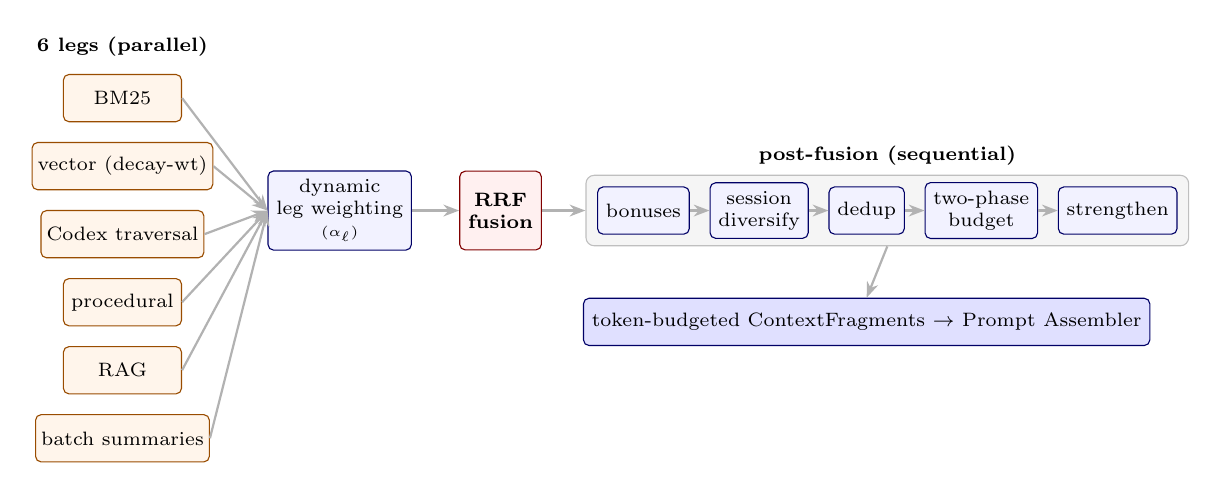
\begin{tikzpicture}[node distance=2.5mm]
% Six legs stacked
\node[iceleg] (l1) {BM25};
\node[iceleg, below=of l1] (l2) {vector (decay-wt)};
\node[iceleg, below=of l2] (l3) {Codex traversal};
\node[iceleg, below=of l3] (l4) {procedural};
\node[iceleg, below=of l4] (l5) {RAG};
\node[iceleg, below=of l5] (l6) {batch summaries};
\node[font=\scriptsize\bfseries, above=1mm of l1] {6 legs (parallel)};
% Weighting
\node[icebox, right=8mm of l3, yshift=3mm, minimum height=10mm] (wt) {dynamic\\leg weighting\\{\tiny($\alpha_\ell$)}};
% RRF
\node[icecore, right=6mm of wt, minimum height=10mm] (rrf) {RRF\\fusion};
% Post-fusion transforms (sequential)
\node[icebox, right=7mm of rrf] (t1) {bonuses};
\node[icebox, right=2.5mm of t1] (t2) {session\\diversify};
\node[icebox, right=2.5mm of t2] (t3) {dedup};
\node[icebox, right=2.5mm of t3] (t4) {two-phase\\budget};
\node[icebox, right=2.5mm of t4] (t5) {strengthen};
\begin{scope}[on background layer]
\node[icephase, fit=(t1)(t5), inner sep=4pt, label={[font=\scriptsize\bfseries]above:post-fusion (sequential)}] (post) {};
\end{scope}
% Output
\node[icebox, fill=blue!12, below=8mm of t3, minimum width=30mm] (out) {token-budgeted ContextFragments $\rightarrow$ Prompt Assembler};
% Arrows legs -> weighting
\foreach \l in {l1,l2,l3,l4,l5,l6} \draw[iceflow] (\l.east) -- (wt.west);
\draw[iceflow] (wt) -- (rrf);
\draw[iceflow] (rrf) -- (post);
\draw[iceflow] (t1) -- (t2); \draw[iceflow] (t2) -- (t3);
\draw[iceflow] (t3) -- (t4); \draw[iceflow] (t4) -- (t5);
\draw[iceflow] (post.south) -- (out.north);
\end{tikzpicture}%
}
\caption{Retrieval orchestrator flow. The six legs are heterogeneous in their retrieval semantics; RRF is the only mechanism that allows them to be combined without score-distribution normalisation; the two-phase token budget guarantees leg diversity under budget pressure.}
\label{fig:orchestrator}
\end{figure}

\subsection{Prompt Assembly}

The Prompt Assembler concatenates the retrieved fragments with persistent memory slots, recent turns, and the live user message into a list of chat-completion messages. The ordering is deliberately \emph{stable-prefix} to maximise KV-cache reuse: (i)~a fixed system message with an inline \texttt{=== PERSISTENT CONTEXT ===} block rendering each active slot; (ii)~recent turns (alternating user/assistant pairs, dynamic per-turn word caps); (iii)~a single user message with header \texttt{=== RETRIEVED CONTEXT ===} (optionally tagged with cluster names when cluster scope is populated); (iv)~a single assistant ``acknowledgment'' message that acts as a boundary marker so the model treats the final user message as the live question rather than another history turn; (v)~the live user question. Because the system message, slots, and most of the recent-turns prefix change slowly, most of the prefix K/V tensors are reusable across consecutive requests.

A two-layer budget process enforces the final size: the orchestrator's \texttt{\_enforce\_token\_budget} packs fragments to \texttt{max\_retrieval\_tokens}, and the API layer recomputes total\_words against a per-model ceiling (2{,}770 words for the deployed model) and iteratively pops procedural and episodic fragments until the budget is met, while preserving RAG and Codex fragments because they are the hardest to recompute and the most likely to carry the answer.

The self-maintaining background worker cluster (fourteen scheduled and event-triggered workers) and the operational infrastructure (FastAPI service, PostgreSQL/pgvector substrate, Celery/Redis worker fleet, and configuration system) are described in Appendix~\ref{app:workers}. A complete technical reference---including the full training pipeline for the classifier and NER models, the controlled relation vocabulary in its entirety, GPU resource management, and idempotency architecture---is available in the technical report archived in the repository (\texttt{docs/ICE\_Architecture[real\_v2].md}), which describes the system at the tagged evaluation snapshot.

%======================================================================
\section{Experimental Design}
\label{sec:exp-design}

\subsection{Why LSREP Was Needed: The Experiment 0 Story}

Our first evaluation attempt (\emph{Experiment 0}) used a precision-based approach: measure whether retrieved fragments contained the relevant information. We constructed probes from a corpus of 41 conversations and asked: did the orchestrator retrieve the fragment with the exact timestamp or ID mapped in the ground-truth file? This failed for two compounding reasons. The first was what we now call the \emph{stateless pronoun problem}---held-out probes were extracted from their original conversations and tested in a vacuum, stripped of surrounding turns; a probe like \emph{``you mentioned that the current script saves nothing''} was fed to the orchestrator with zero surrounding context, so the system pulled fragments that were mathematically correct in isolation but functionally useless. The second was the \emph{incompetent judge}---a 7B grading model that hallucinated failures, scoring 0 for fragments a human immediately recognised as the exact brainstorming session being asked about. Manual re-scoring on a subset of the probes produced 31\% precision rather than the automated 13.87\%, and the gap was attributable to the judge, not the retrieval system.

The failure of the stateless precision benchmark led directly to the idea of LSREP. If a weak judge could not be trusted to score fragments, the system needed to be asked to answer real questions, and the answers themselves needed to be judged. And if memory accumulation was to be measured, the same questions needed to be asked at multiple points in time, not just once at the end. The first sketch was: replay a conversation from the beginning, pause at regular intervals, ask hand-written questions, and score the answers against the full conversation history. That sketch became LSREP.

\subsection{LSREP: The General Protocol}
\label{sec:lsrep}

LSREP freezes a historical conversation at an arbitrary temporal slice $T_n$, reconstructs the entire database and memory-lifecycle state exactly as it existed at that moment, injects evaluation probes, and then evaluates the system's answers with an independent judge. Its defining choice is to evaluate the \emph{model's output}, not the retrieval pipeline's intermediate results---because a fragment that is ``irrelevant'' at turn 100 may become critically relevant at turn 800, and a fragment that differs from the ground truth may still be \emph{equally valid} (the multiple-correct-answer problem that sank Experiment 0).

The general procedure is: for each historical conversation, determine the total turn count $L$ and select split points; wipe the target database and inject turns $T_1$ through $T_{n-1}$ sequentially into the episodic memory tables, preserving exact relative or real timestamps; trigger the background workers synchronously (decay computes initial \texttt{decay\_score} metrics, the codex extractor builds entity nodes and relationship edges, the procedural extractor scans for behavioural motifs, and the clustering worker aggregates related turns); then administer the probes and judge the answers.

This skeleton is common to both experiments. \emph{However, the two experiments instantiate it very differently}---in split range, probe construction, ground-truth generation, checkpoint handling, and the evaluated system itself. Because those differences are large enough to affect how the results should be read, we describe each experiment's environment separately below, and summarise the differences in \cref{tab:exp-diff}. A single caveat frames everything that follows: \textbf{Experiment 1 is a pilot}. Its role was to expose measurement flaws and immature subsystems; the paper's substantive evaluation is Experiment 2, and Experiment 3 is the ablation that explains \emph{why} the mature system behaves as it does.

\subsection{Experiment 1 Environment (Pilot)}
\label{sec:exp1-env}

\textbf{System under test.} Experiment 1 evaluated an immature build with only the vector and BM25 retrieval legs meaningfully active. The classifier used a frozen MiniLM (\texttt{all-MiniLM-L6-v2}) embedding backbone; retrieval used static per-leg limits and a static global token budget (5{,}000 tokens) plus an uncapped 10-turn sliding window; the Codex knowledge graph effectively did not exist yet (a regex tagger and an under-powered 1.5B extractor produced almost no usable edges), so ICE's graph, procedural, and document legs contributed nothing and the system reduced to essentially the same vector\,$+$\,BM25 retrieval as the baseline; and cluster-scoped retrieval did not yet exist. Two of these---the static budget and the uncapped sliding window---directly caused the token-accounting problem described below.

\textbf{Protocol instantiation.} Conversations shorter than 10 turns were excluded, reducing the corpus from 42 (the Experiment 0 corpus) to 18. Split points were drawn from $[\max(10,0.30L),\,0.95L]$, three per conversation with a fixed seed; each split defined a historical block (turns $1..s$) and a future reference block (the next 10 turns). Probes were \emph{hand-written}, 8--30 per conversation, and probes from earlier splits were re-asked at later splits to observe change over time. Ground truth used a \emph{single} retrieval-assisted pass: the probe was embedded, similar turns retrieved (20--40 turns, 30{,}000-token cap), and a language model compiled the retrieved evidence into one reference answer---frozen for that probe. Six conditions were run per probe (two control / sliding-window-only, two vector-RAG, two Full ICE, each in generalist and MoE variants).

\textbf{The token-accounting audit.} After Experiment 1 completed, an audit found that the reported context size for Full ICE included retrieved fragments but \emph{omitted} the recent-turn sliding window incorporated during prompt assembly. The generated answers, scores, rankings, and hallucination labels were unaffected---the sliding window was correctly supplied to the model at inference time; only the reported context-efficiency statistics were wrong. We replayed the sliding-window assembly (10 turns, 500-word-per-turn cap) for every checkpoint and added the omitted tokens. The correction did not change the qualitative findings, but it did invalidate any claim of superior token efficiency: corrected, Full ICE consumes \emph{more} total tokens than the vector baseline at roughly equal quality. Experiment 1 is therefore a proof-of-concept for memory quality and retrieval behaviour, not a demonstration of context compression. This finding directly motivated Experiment 2's unified dynamic token budget. All Experiment 1 numbers reported in this paper are the corrected values.

\subsection{Experiment 2 Environment (Mature System)}
\label{sec:exp2-env}

\textbf{System under test.} Experiment 2 evaluated the mature system: the classifier backbone was upgraded to Qwen3-Embedding-0.6B and the head retrained from scratch; a trained Micro-NER model replaced Experiment~1's regex entity tagger, so the Codex extractor now grounds on real entity detection ($\sim$95\% recall); a conservative routing override was added (favour retrieval under low confidence or long conversations); the static budget and uncapped sliding window were replaced by the unified \emph{dynamic} token budget of Section~\ref{sec:architecture}; and \emph{cluster-scoped retrieval} was introduced, restricting episodic search to the most relevant topical clusters rather than the whole conversation. These changes are the reason Experiment 2 can inject fewer fragments while holding quality: the gain comes from cleaner, more focused evidence, not more of it.

\textbf{Protocol instantiation.} Rather than many conversations at isolated checkpoints, Experiment 2 followed four carefully chosen long-horizon conversations (Section~\ref{sec:datasets}) across their entire lifespan. Three instantiation choices differ sharply from Experiment 1. \emph{(1)~Continuous replay with preserved state}: each conversation was replayed chronologically into one fresh deployment, and memory stored at an early checkpoint remained available at every later checkpoint (in Experiment 1 each checkpoint was effectively independent). A simulated memory lifecycle---decay, codex-edge decay, procedural decay, reflection, clustering, consolidation, sentinel monitoring---ran \emph{between} checkpoints so retrieval reflected aged, consolidated memory rather than fresh storage. \emph{(2)~Automatic, retrieval-leg-aware probe generation}: probes were generated at each checkpoint from a sampled history window (first 5 turns, last 10 before the checkpoint, 15 random from between), using only information available up to that checkpoint, and were explicitly targeted at specific legs (Codex, vector, BM25, procedural). Every probe required a unique temporal anchor to prevent ambiguity across hundreds of turns. These auto-generated probes were combined with the 72 hand-written probes inherited from Experiment 1. \emph{(3)~Incremental evaluation}: every probe whose origin was at or before a checkpoint was re-evaluated at that checkpoint, so a probe generated early is scored repeatedly as history accumulates---which is what makes longitudinal memory growth directly observable.

\textbf{Evolving ground truth.} The single frozen ground truth of Experiment 1 was replaced by a three-stage temporal-refinement pipeline: \emph{(i)~forensic regeneration} of the origin-checkpoint answer under a stricter, evidence-oriented prompt that records temporal provenance and distinguishes historical from current state; \emph{(ii)~temporal anchoring}, attaching to each probe an anchor identifying the specific fact/event it tracks; and \emph{(iii)~forward propagation}, updating each answer at every later checkpoint when new content contradicts, updates, or extends it, while anchor-preservation checks guard against silent drift to a superficially similar later event. The result is that each probe carries a \emph{temporally evolving} reference document rather than a static answer---necessary because otherwise a system that correctly \emph{updated} a fact could score worse than one that repeated an outdated fact.

\textbf{Scoring differences.} Experiment 2 added temporal-aware scoring (an answer can lose points for reporting a superseded fact even if it was once correct) and inference credit (a specific, evidence-consistent detail not explicitly in the reference is rewarded, not flagged as hallucination). Structural-relevance assessment credits fragments that provide supporting background without containing the answer verbatim.

\textbf{Human verification, not score alteration.} Two independent pieces of human involvement in Experiment 2 are worth stating precisely, because ``manually verified'' can be misread as ``scores were adjusted by hand.'' They were not; the human role was verification and correction of the judge's own labels, not substitution of human judgment for the judge's. First, the 72 hand-written probes inherited from Experiment 1 (Section~\ref{sec:exp1-env}) were re-evaluated by hand against their absolute scores and tournament rankings, so a genuine human-authored, human-checked evaluation slice sits inside the Experiment 2 benchmark alongside the automatically generated and automatically judged probes---not merely the model's own self-consistency. Second, every hallucination flag across all 1{,}211 probes was manually audited. This second correction was necessary because the automated judge was systematically too harsh across \emph{all four} conditions---generalist and MoE, ICE and vector alike---whenever an answer contained a specific, true, and directly relevant detail that was simply absent from the necessarily condensed ground-truth dossier; the judge tended to flag such details as unsupported rather than recognise them as correct supplementary information. The audit corrected these false positives wherever a detail was verifiably true against the source conversation, applying the same standard to every condition; it did not remove flags for genuine fabrications, and we deliberately did not over-correct in the other direction by crediting speculative or unverifiable additions. This audit was applied to Experiment 2 only; Experiment 3 (the ablation) uses the automated judge's hallucination labels unmodified, for the bias reasons discussed in Section~\ref{sec:limitations}.

\textbf{Ground-truth and judge.} Both experiments use the same independent judge, \texttt{mattbucci/gemma-4-12B-AWQ} on SGLang (150{,}000-token context, temperature 0.0, deterministic decoding), never used for retrieval, generation, probe generation, or ground-truth construction. The extraction rules---Strict Neutrality, Verbatim Anchor Preservation, Temporal Dominance, Third-Person Attribution---are shared; what differs is that Experiment 2 applies them through the evolving-dossier pipeline above rather than a single pass.

\begin{table}[htbp]
\centering
\small
\caption{What differs between the two LSREP instantiations. Experiment 1 is a pilot; Experiment 2 is the paper's substantive evaluation. The shared skeleton (state reconstruction, synchronous worker trigger, output-level judging by the same independent judge) is described in Section~\ref{sec:lsrep}.}
\label{tab:exp-diff}
\begin{tabular}{@{}L{3.3cm}L{5.0cm}L{5.0cm}@{}}
\toprule
\textbf{Dimension} & \textbf{Experiment 1 (Pilot)} & \textbf{Experiment 2 (Mature)} \\
\midrule
System maturity & Vector + BM25 legs; MiniLM classifier; static budget; uncapped sliding window; Codex non-functional & Six legs; Qwen3 classifier + routing override; dynamic budget; cluster-scoped retrieval \\
Corpus & 18 conversations (isolated checkpoints) & 4 long-horizon conversations (full-lifespan replay) \\
Split range & $[\max(10,0.30L),\,0.95L]$, 3 splits/conv & Length-adaptive checkpoints (8--20), even spacing with jitter \\
Probes & Hand-written (8--30/conv) & Auto-generated + leg-aware (147) plus 72 inherited hand-written \\
Ground truth & Single retrieval-assisted pass, \emph{frozen} & Three-stage forensic regeneration + forward propagation, \emph{evolving} \\
Checkpoint state & Independent per checkpoint & Preserved across checkpoints; lifecycle runs between them \\
Probe evaluation & Each probe once & Incremental: re-scored at every later checkpoint \\
Scoring & Static correctness & Temporal-aware + inference credit; hallucination flags audited for false positives \\
Conditions & Six (incl.\ sliding-window controls) & Four (controls dropped) \\
\bottomrule
\end{tabular}
\end{table}

\textbf{Evaluation conditions (Experiment 2).} The mature evaluation used a four-condition matrix: \textbf{Vector RAG Baseline (Generalist)}---single-leg pgvector similarity, top-K=30, no decay weighting, classification, or fusion, generalist model (\texttt{gemma4:26b-a4b-it-q4\_K\_M}); \textbf{Vector RAG Baseline (MoE)}---same retrieval, expert-routed; \textbf{Full ICE (Generalist)}---all six legs, RRF fusion, classification, decay weighting, dynamic budget, post-fusion processing; and \textbf{Full ICE (MoE)}---same ICE retrieval, expert-routed. The vector baseline is a standard single-leg vector-RAG---the top-30 similar turns assembled with the question---while the ICE conditions run the full system: fused multi-leg retrieval plus ICE's prompt assembler (persistent memory slots, a recent-turns window, structured boundaries). Both use the same embedder and database. The comparison is therefore \emph{full memory system versus standard vector-RAG}: ICE's curation deliberately governs \emph{what} context is assembled, not merely which fragments are retrieved. (At the snapshot the multi-leg configuration reduced in practice to the two episodic legs plus a small Codex share; Section~\ref{sec:limitations}.) The sliding-window-only control conditions from Experiment 1 were dropped, having already been characterised.

\textbf{A note on conservatism.} Because history is \emph{replayed} rather than lived, the reinforcement that normally strengthens frequently-referenced memories during live use is largely absent---the primary reinforcement signal becomes the evaluation probes themselves. A concept referenced dozens of times in real use and one mentioned once therefore look more alike under replay than they would in deployment. Experiment 2's numbers should thus be read as a conservative lower bound on deployed performance, not a ceiling (see Section~\ref{sec:limitations}).

\subsection{Metrics}

\begin{table}[htbp]
\centering
\small
\caption{Evaluation metrics. Each metric is computed per probe and aggregated across the benchmark.}
\label{tab:metrics}
\begin{tabular}{p{0.20\columnwidth}p{0.42\columnwidth}p{0.30\columnwidth}}
\toprule
\textbf{Metric} & \textbf{Definition} & \textbf{What it measures} \\
\midrule
Score (1--5) & Mean absolute score from the judge & Answer quality \\
SPF (Score per Fragment) & $\mathrm{mean\_score} / \mathrm{mean\_fragments}$ & Retrieval efficiency \\
TUR (Token Utilisation Rate) & $\mathrm{mean\_score} / (\mathrm{mean\_tokens}/1000)$ & Token efficiency \\
Win Rate (\%) & Blind tournament ranking: all four conditions' answers for a probe are anonymised, shuffled, and ranked best-to-worst by the judge in a single pass, independent of the absolute (1--5) scoring; win rate is the share of tournament appearances placed first & Relative preference, judge-order-bias-free \\
Hallucination (\%) & Percentage of probes where the judge detects fabricated information not present in the conversation & Faithfulness \\
Fragment Count & Mean fragments injected per probe & Retrieval volume \\
Recency Delta & $\mathrm{mean\_score}(\mathrm{late\ bins}) - \mathrm{mean\_score}(\mathrm{early\ bins})$ & Longitudinal improvement \\
\bottomrule
\end{tabular}
\end{table}

No single metric captures memory quality, which is why we report several and read them together. Absolute \emph{score} measures answer quality but conceals the cost at which it was achieved; \emph{SPF} and \emph{TUR} expose that cost (quality per fragment, and per thousand injected tokens), which is the axis on which a curated memory system must distinguish itself from a firehose that simply retrieves more. \emph{Win rate} is the noise-robust relative signal: a blind tournament ranking sidesteps the absolute-scale drift that makes raw 1--5 judgments hard to compare across hundreds of probes, so it often separates systems that tie on mean score. \emph{Hallucination} and \emph{fragment count} guard the two ways a system can look good on score yet fail in practice---fabrication, and context bloat. \emph{Recency delta} is the longitudinal signal unique to this setting: whether answers \emph{improve} as memory accumulates over the conversation, which a static-corpus baseline structurally cannot exhibit. Together these separate ``answers well'' from ``answers well while staying efficient, faithful, and improving over time.''

Where confidence intervals are reported, they are 95\% percentile-bootstrap intervals computed by resampling probes with replacement (10{,}000 resamples) over the same per-probe records that produce the point estimates, including the published missing-score imputation; paired score differences are computed within-probe before resampling.

%======================================================================
\section{Results}
\label{sec:results}

\subsection{Pilot Studies: Experiment 0 and Experiment 1}
\label{sec:exp1}

\textbf{Experiment 0} (precision-based evaluation) failed for the reasons described in Section~\ref{sec:exp-design}: stateless probes penalised accurate context-dependent retrieval, and a weak 7B judge hallucinated failures. The manually re-scored 31\% precision confirmed that the gap was the judge, not the retrieval. This failure taught us that evaluating retrieval intermediates is the wrong level of abstraction---we must evaluate model outputs---and led directly to LSREP.

\textbf{Experiment 1} (``Infant Metabolism'') was the first full LSREP run, using the pilot environment of Section~\ref{sec:exp1-env}: the immature system (vector + BM25 legs, MiniLM classifier, static budget, non-functional Codex), 18 conversations at isolated checkpoints, hand-written probes, and a single frozen ground truth. It was evaluated on 657 probes. After the token-accounting audit described in Section~\ref{sec:exp1-env}, the corrected numbers tell a sobering story. \cref{tab:exp1} shows the six-core benchmark with corrected token counts. \emph{We report Experiment 1 not as a result but as a pilot}---its value is diagnostic, and Experiment 2 (Section~\ref{sec:exp2}) is the paper's substantive evaluation.

\begin{table}[htbp]
\centering
\small
\caption{Experiment 1 (Immature System) --- Six-core benchmark, 657 probes, corrected token counts. After correcting the sliding-window under-count, ICE used more tokens than the vector baseline, scored slightly lower, hallucinated more, and had a worse TUR. The system was not yet a fair test of the architecture.}
\label{tab:exp1}
\begin{tabular}{@{}lrrrrr@{}}
\toprule
\textbf{Condition} & \textbf{Score} & \textbf{Tokens} & \textbf{Hall.\ (\%)} & \textbf{TUR} & \textbf{Win \%} \\
\midrule
Control Baseline (Generalist) & 3.05 $\pm$ 1.61 & 3{,}998  & 74.1 & 0.76 & 11.3 \\
Control MoE                   & 3.01 $\pm$ 1.61 & 3{,}998  & 74.4 & 0.75 & 7.6  \\
Vector RAG (Generalist)       & \textbf{4.06} $\pm$ 1.31 & \textbf{5{,}847}  & \textbf{64.7} & \textbf{0.69} & 22.9 \\
Vector RAG (MoE)              & 4.05 $\pm$ 1.32 & 5{,}847  & 66.7 & 0.69 & 15.6 \\
\textbf{Full ICE (Generalist)}& 4.04 $\pm$ 1.33 & 8{,}586  & 69.6 & 0.47 & 22.0 \\
\textbf{Full ICE (MoE)}       & 3.96 $\pm$ 1.33 & 8{,}586  & 72.3 & 0.46 & 20.6 \\
\bottomrule
\end{tabular}
\end{table}

The full ICE generalist scored 4.04 against the vector baseline's 4.06, used 47\% more tokens (8{,}586 vs 5{,}847), hallucinated more (69.6\% vs 64.7\%), and posted a worse TUR (0.47 vs 0.69). The MoE variant was worse still (3.96). The picture brightened slightly on the longitudinal axis---193 tracked question curves showed scores improving over time on repeated probes, demonstrating memory accumulation---but the headline numbers were a defeat. Several subsystems were broken or immature: only 3 decay cycles had run; the Codex knowledge graph effectively did not exist (a regex tagger and under-powered 1.5B extractor yielded almost no usable edges), so ICE was essentially vector\,$+$\,BM25 retrieval---barely distinguishable from the baseline; 22 gating failures meant the classifier was actively blocking retrieval on probes that needed it; the sliding-window under-count had to be corrected after the fact; and the token budget was static, not dynamic.

\textbf{Lessons learned.} A system that has not had time to consolidate memory is not a fair test. Honest token counting is essential---the sliding-window under-count was a measurement bug that, left uncorrected, would have made ICE look more efficient than it was. And a broken subsystem (Codex, NER) can drag down the entire system, which is itself an important finding about the fragility of multi-component architectures. Experiment 1 was not published as a standalone result; it served as a pilot that revealed every measurement flaw and system immaturity that needed to be addressed before a fair evaluation could be run.

\subsection{Mature System Evaluation (Experiment 2)}
\label{sec:exp2}

Experiment 2 focused on four long-form conversations. \cref{tab:exp2-global} reports the four conditions on the three-conversation ``fair comparison'' view (Dataset C / Technical Planning excluded; 1{,}057 probes). \cref{tab:exp2-perconv} breaks the results down by conversation. \cref{tab:exp2-score-dist} shows the score distribution, and \cref{tab:exp2-temporal} groups the scores by quality bucket.

\begin{table}[htbp]
\centering
\small
\caption{Experiment 2 (Mature System) --- Global comparison, ICE-Dev excluded (1,057 probes across 3 conversations). On the three conversations where both systems could actually generate usable answers, ICE essentially ties the vector baseline on mean score (4.26 vs 4.25), injects 32\% fewer fragments, and wins 30.6\% of head-to-head comparisons (vs 21.2\%).}
\label{tab:exp2-global}
\resizebox{\textwidth}{!}{%
\begin{tabular}{@{}lccccccc@{}}
\toprule
\textbf{Condition} & \textbf{Score} & \textbf{Tokens} & \textbf{Frags} & \textbf{SPF} & \textbf{TUR} & \textbf{Win \%} & \textbf{Hall. \%} \\
\midrule
Vector RAG Generalist & 4.25 $\pm$ 1.09 & 21{,}025 & 30.0 & 0.14 & 0.20 & 21.2 & 20.5 \\
Vector RAG MoE        & 4.24 $\pm$ 1.04 & 21{,}025 & 30.0 & 0.14 & 0.20 & 19.2 & 17.4 \\
Full ICE Generalist   & 4.26 $\pm$ 1.08 & 22{,}411 & 20.4 & 0.21 & 0.19 & \textbf{30.6} & 19.6 \\
Full ICE MoE          & \textbf{4.28} $\pm$ 0.99 & 22{,}411 & 20.4 & 0.21 & 0.19 & 29.0 & 19.9 \\
\bottomrule
\end{tabular}%
}
\end{table}

\begin{table}[htbp]
\centering
\small
\caption{Experiment 2 --- Per-conversation breakdown (generalist conditions). ICE wins more head-to-head comparisons on every conversation. On Dataset A (Creative Writing) ICE's win rate (37.2\%) is more than double the vector baseline's (18.0\%).}
\label{tab:exp2-perconv}
\resizebox{\textwidth}{!}{%
\begin{tabular}{@{}lrrrrrr@{}}
\toprule
\textbf{Dataset} & \textbf{ICE Score} & \textbf{Vec. Score} & \textbf{ICE Tok.} & \textbf{Vec. Tok.} & \textbf{ICE Win \%} & \textbf{Vec. Win \%} \\
\midrule
Dataset A (Creative Writing)  & 3.63 & 3.50 & 19{,}434 & 24{,}360 & \textbf{37.2} & 18.0 \\
Dataset B (Long-Form Creative) & 4.28 & 4.33 & 24{,}108 & 21{,}257 & 32.8 & 22.9 \\
Dataset D (Academic Planning)  & \textbf{4.63} & 4.57 & 20{,}103 & 18{,}076 & 20.4 & 18.8 \\
\bottomrule
\end{tabular}%
}
\end{table}

\begin{table}[htbp]
\centering
\small
\caption{Experiment 2 --- Score distribution (1,057 probes, ICE-Dev excluded). The full distribution shows that the mean-score tie masks a structural difference: ICE-MoE has the lowest score-1 rate (1.5\%) but shifts mass from score-5 to score-3/4, producing a lower-variance output.}
\label{tab:exp2-score-dist}
\begin{tabular}{rrrrr}
\toprule
\textbf{Score} & \textbf{ICE Gen (\%)} & \textbf{ICE MoE (\%)} & \textbf{Vec. Gen (\%)} & \textbf{Vec. MoE (\%)} \\
\midrule
1 (poor)      & 3.0 & 1.5 & 3.8 & 2.4 \\
2             & 5.9 & 4.3 & 4.3 & 3.9 \\
3 (acceptable)& 13.3 & 16.6 & 14.8 & 19.5 \\
4 (good)      & 18.1 & 19.7 & 17.2 & 16.3 \\
5 (excellent) & 59.7 & 58.0 & 60.0 & 58.0 \\
\bottomrule
\end{tabular}
\end{table}

\begin{table}[htbp]
\centering
\small
\caption{Experiment 2 --- Temporal score quality (1,057 probes, ICE-Dev excluded). Quality buckets: Good (4--5), OK (3), Poor (1--2). ICE-Generalist has the highest Good rate (77.8\%) among the four conditions.}
\label{tab:exp2-temporal}
\begin{tabular}{lrrr}
\toprule
\textbf{Condition} & \textbf{Good (4--5) \%} & \textbf{OK (3) \%} & \textbf{Poor (1--2) \%} \\
\midrule
Vector RAG Generalist  & 77.2 & 14.8 & 8.0 \\
Vector RAG MoE         & 74.3 & 19.5 & 6.2 \\
Full ICE Generalist    & \textbf{77.8} & 13.3 & 8.9 \\
Full ICE MoE           & 77.7 & 16.6 & 5.8 \\
\bottomrule
\end{tabular}
\end{table}

The mean-score difference between ICE Generalist and Vector Generalist is +0.01 (4.26 vs 4.25). A paired per-probe bootstrap (10{,}000 resamples over the 1{,}057 probes; both conditions answer the same probes, so the difference is computed within-probe) places this difference at $+0.00$ with a 95\% confidence interval of $[-0.07, +0.07]$: a genuine, tightly-estimated statistical tie, not an ambiguous one. Several secondary metrics tell a more interesting story. ICE injects 32.0\% fewer fragments (20.4 vs 30.0) while achieving the same quality, giving an SPF of 0.21 vs 0.14 (a 50\% improvement in efficiency per fragment). The head-to-head win rate is the cleanest signal, and it is statistically robust: ICE Generalist wins 30.6\% of tournament appearances (95\% CI $[27.9, 33.4]$) against the vector baseline's 21.2\% ($[18.8, 23.7]$)---the intervals do not overlap. When the systems disagree, ICE is more likely to be right. ICE uses 6.6\% more tokens (22{,}411 vs 21{,}025) because its fragments are higher-quality and longer on average, but it uses them in a more compact set. Hallucination rates are roughly equal (19.6\% vs 20.5\%).

\textbf{Leg contributions} (ICE Generalist): episodic 62.3\%, codex 3.3\%, unknown (fragments whose source leg could not be reconstructed) 34.5\%. The codex contribution is small but targeted---and the 3.3\% figure additionally \emph{undercounts} the Codex's share of injected content by construction: the evaluated implementation collapsed an entire graph traversal (every visited entity and its context payload) into a \emph{single} concatenated fragment per probe, whereas the episodic legs emit each turn as its own fragment. A Codex contribution carrying a dozen entities therefore counted as one fragment against dozens of individually-counted episodic fragments, and could occupy at most one slot in token-budget enforcement regardless of relevance. The fragment-share metric is thus a lower bound on the Codex's content share, not a measure of it. \textbf{Fragment--score correlation} reveals a qualitative difference: ICE Generalist shows $r = +0.193$ (MoE: $+0.246$), while Vector Generalist shows $r = -0.015$ (MoE: $-0.030$). For ICE, retrieving more fragments correlates with better answers; for the vector baseline, retrieving more fragments correlates with worse answers---a strong signal that ICE's fragments carry signal while the vector baseline's carry noise.

\textbf{Per-conversation results} vary by domain. On Dataset A (Creative Writing), ICE's win rate is more than double the vector baseline's (37.2\% vs 18.0\%). On Dataset B (Long-Form Creative Writing), the largest conversation at 1{,}119 turns, the vector baseline actually wins on mean score (4.33 vs 4.28) but ICE wins on win rate (32.8\% vs 22.9\%) and uses 18\% more tokens because it serves more detailed, complete answers. On Dataset D (Academic Planning), ICE wins on both mean score (4.63 vs 4.57) and win rate (20.4\% vs 18.8\%). \textbf{Longitudinal score evolution.} \cref{fig:longitudinal} shows how the mean probe score evolves across turn-index bins for the four conditions on the three-conversation view. All four conditions track closely through the early and middle bins---the mean-score tie is visible as four largely overlapping curves. The decisive separation appears at the deepest long-horizon bin (turn 1{,}100 of Dataset B): both vector conditions drop sharply to 3.80 (generalist) and 3.87 (MoE), while both ICE conditions hold at 4.18 (generalist) and 4.14 (MoE). The vector baseline is not using the long-tail knowledge that ICE has consolidated; its retrieval cannot reach across 1{,}000+ turns of conversation history, and the gap opens precisely where that reach matters.

\begin{figure}[t]
\centering
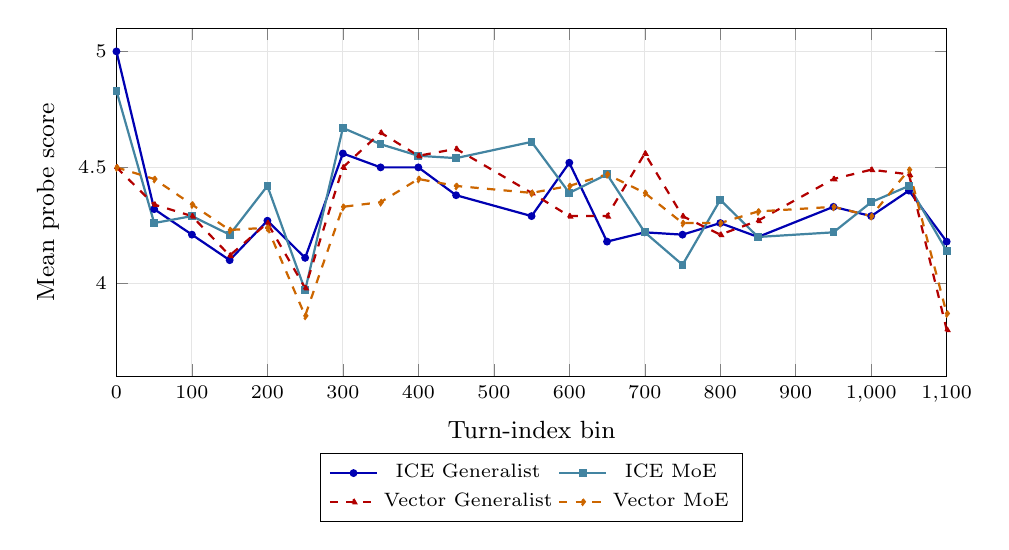
\begin{tikzpicture}
\begin{axis}[
    width=\columnwidth, height=6cm,
    xlabel={\small Turn-index bin}, ylabel={\small Mean probe score},
    ylabel near ticks,
    xmin=0, xmax=1100, ymin=3.6, ymax=5.1,
    tick label style={font=\scriptsize},
    legend style={font=\scriptsize, at={(0.5,-0.22)}, anchor=north, legend columns=2},
    grid=major, grid style={gray!20},
]
\addplot[blue!70!black, thick, mark=*, mark size=1pt] coordinates
 {(0,5) (50,4.32) (100,4.21) (150,4.1) (200,4.27) (250,4.11) (300,4.56) (350,4.5) (400,4.5) (450,4.38) (550,4.29) (600,4.52) (650,4.18) (700,4.22) (750,4.21) (800,4.26) (850,4.2) (950,4.33) (1000,4.29) (1050,4.4) (1100,4.18)};
\addplot[cyan!60!black, thick, mark=square*, mark size=1pt] coordinates
 {(0,4.83) (50,4.26) (100,4.29) (150,4.21) (200,4.42) (250,3.97) (300,4.67) (350,4.6) (400,4.55) (450,4.54) (550,4.61) (600,4.39) (650,4.47) (700,4.22) (750,4.08) (800,4.36) (850,4.2) (950,4.22) (1000,4.35) (1050,4.42) (1100,4.14)};
\addplot[red!70!black, thick, dashed, mark=triangle*, mark size=1pt] coordinates
 {(0,4.5) (50,4.34) (100,4.29) (150,4.12) (200,4.26) (250,3.98) (300,4.5) (350,4.65) (400,4.55) (450,4.58) (550,4.39) (600,4.29) (650,4.29) (700,4.56) (750,4.29) (800,4.21) (850,4.27) (950,4.45) (1000,4.49) (1050,4.47) (1100,3.8)};
\addplot[orange!80!black, thick, dashed, mark=diamond*, mark size=1pt] coordinates
 {(0,4.5) (50,4.45) (100,4.34) (150,4.23) (200,4.24) (250,3.86) (300,4.33) (350,4.35) (400,4.45) (450,4.42) (550,4.39) (600,4.42) (650,4.47) (700,4.39) (750,4.26) (800,4.26) (850,4.31) (950,4.33) (1000,4.29) (1050,4.49) (1100,3.87)};
\legend{ICE Generalist, ICE MoE, Vector Generalist, Vector MoE}
\end{axis}
\end{tikzpicture}
\caption{Longitudinal mean score by turn-index bin (1{,}057 probes, ICE-Dev excluded; real per-bin data). All four conditions track closely through the mid-conversation bins, but at the final turn-1{,}100 bin---the deep long-horizon regime of Dataset B---both vector conditions drop sharply (to 3.80 generalist, 3.87 MoE) while both ICE conditions hold (4.18 generalist, 4.14 MoE). The divergence at the extreme horizon is the practical advantage of ICE's consolidated long-tail memory.}
\label{fig:longitudinal}
\end{figure}

\textbf{MoE vs.\ generalist.} The global MoE-vs-generalist score delta is +0.01 for ICE and $-$0.02 for vector; the effect is too small to claim a meaningful advantage in either direction. MoE provides a modest 3.1\% hallucination reduction under vector but a $-$0.3\% hallucination increase under ICE. MoE provides no token savings. The MoE infrastructure is therefore architecturally present but empirically neutral in this evaluation---a finding we return to in the Discussion.

\textbf{Memory maturity} is reported per conversation: Dataset B had 93 simulated decay days at its final checkpoint, Dataset A had 24, Dataset C had 27, Dataset D had 20. Gating failures dropped from 22 in Experiment 1 to 2 in Experiment 2---the single largest reliability improvement in the entire mature deployment.

\textbf{Human-verified slice.} The 72 hand-written probes inherited from Experiment~1 were scored entirely by hand---both an absolute 1--5 score and a blind, anonymised tournament ranking---giving a human-authored, human-judged slice inside the benchmark (\cref{tab:manual}). On this slice the picture is far less equivocal than the automated tie: both ICE conditions score ${\sim}4.3$ against the baselines' ${\sim}3.1$, and the paired ICE-minus-baseline difference is $+1.21$ (95\% CI $[+0.81, +1.61]$), decisively excluding zero. Two readings are consistent with this, and we lean on neither. The optimistic one: the automated judge---shown in Section~\ref{sec:limitations} to be systematically harsh---\emph{understates} ICE's advantage, so the headline tie is a conservative lower bound. The cautious one: these 72 are the harder, more memory-dependent, author-written questions on which stored context matters most, and a single scorer (even blinded per probe) cannot be assumed unbiased. The human slice's dependable value is narrower but real---it is an independent check that the automated tie is not concealing an ICE \emph{deficit}. The within-ICE tournament asymmetry (the MoE variant taking 69.4\% of first-place ranks despite a marginally lower mean) is not stable at this sample size and should not be read as an MoE effect.

\begin{table}[htbp]
\centering
\small
\caption{Human-verified slice (72 hand-scored probes, independent of the automated judge). ICE beats the vector baseline decisively here---paired ICE-vs-Vector $= +1.21$ (95\% CI $[+0.81, +1.61]$)---in contrast to the automated tie over all 1{,}057 probes, consistent with the automated judge being conservative. Single-scorer; blind per-probe tournament ranking.}
\label{tab:manual}
\begin{tabular}{@{}lccc@{}}
\toprule
\textbf{Condition} & \textbf{Score} & \textbf{95\% CI} & \textbf{Win \%} \\
\midrule
Vector RAG (Generalist) & 3.10 & $[2.75, 3.44]$ & 5.6 \\
Vector RAG (MoE)        & 3.22 & $[2.88, 3.54]$ & 8.3 \\
Full ICE (Generalist)   & 4.31 & $[4.11, 4.49]$ & 16.7 \\
Full ICE (MoE)          & 4.24 & $[4.01, 4.43]$ & \textbf{69.4} \\
\bottomrule
\end{tabular}
\end{table}

\textbf{Lessons learned.} The mean-score tie masks an important qualitative difference: ICE wins more head-to-head comparisons and its fragments are positively correlated with answer quality, while the vector baseline's fragments are negatively correlated. The 32\% fragment reduction is the most practically significant finding---it means ICE can achieve the same quality with substantially less context pollution. The MoE finding is the most humbling: an architecturally elaborate component delivers no measurable benefit under realistic conditions.

\subsection{Stress Test: Context Overflow on Dataset C (ICE-Dev)}
\label{sec:stress}

Dataset C (Technical Planning) contains architecture documents that frequently exceed 8{,}000 tokens per turn. The vector baseline, which always retrieves the top-30 fragments with no per-query budget, injects a mean of 88{,}061 tokens (with failed cases reaching 100{,}505), overwhelming the model's context window. Of 154 probes, 145 fail with a score of 1 (a 94.2\% failure rate)---the retrieval subsystem actually found relevant information, but the generation model could not process the assembled context and produced empty or degenerate responses. ICE, with its dynamic token budget and \texttt{\_enforce\_token\_budget} capping retrieval, maintains a mean of 19{,}953 tokens and produces a mean score of 4.33.

\begin{table}[htbp]
\centering
\small
\caption{ICE-Dev stress test (154 probes). The vector baseline collapses to a 94.2\% failure rate on the technical-planning conversation because it has no token-budget cap. ICE survives the same conversation with a mean score of 4.33 and 77\% fewer tokens injected. Note: the vector baseline's 0\% hallucination rate is misleading---94.2\% of its responses are complete failures (score 1), so there is no answer to evaluate for hallucination.}
\label{tab:stress}
\resizebox{\textwidth}{!}{%
\begin{tabular}{@{}lrrrrrrrr@{}}
\toprule
\textbf{Condition} & \textbf{Score} & \textbf{Tok.} & \textbf{Frags} & \textbf{SPF} & \textbf{TUR} & \textbf{Hall \%} & \textbf{Win \%} & \textbf{Overflow \%} \\
\midrule
Vector RAG Generalist & 1.23 & 88{,}061 & 30 & 0.04 & 0.01 & 0.0* & 1.9 & \textbf{94.2} \\
Vector RAG MoE        & 1.10 & 88{,}061 & 30 & 0.04 & 0.01 & 0.0* & 4.5 & 97.4 \\
Full ICE Generalist   & \textbf{4.33} & 19{,}953 & 10 & \textbf{0.43} & \textbf{0.22} & 41.4 & 43.5 & 3.9 \\
Full ICE MoE          & 4.03 & 19{,}953 & 10 & 0.40 & 0.20 & 40.8 & \textbf{50.0} & 16.2 \\
\bottomrule
\end{tabular}%
}
\end{table}

The score distribution on Dataset C is striking. ICE Generalist: 3.9\% at score 1, 5.2\% at 2, 11.7\% at 3, 12.3\% at 4, and 66.9\% at 5---66.9\% of its answers are excellent. The vector baseline: 94.2\% at score 1, 0\% at 2/3/4, and 5.8\% at 5. ICE's SPF is 0.43, more than 10$\times$ the vector baseline's 0.04; the same 0.43 of ``quality per fragment'' would mean 130 fragments for the vector baseline to match ICE's quality, which is structurally impossible.

The 41.4\% hallucination rate for ICE on Dataset C deserves a careful note. ICE is trying to answer a difficult question, and sometimes gets it wrong. The vector baseline is not trying at all (94.2\% of its responses are complete failures), so it never hallucinates. A 0\% hallucination rate here is not evidence of reliability; it is evidence of absence. The 41.4\% hallucination rate reflects the difficulty of the task and the model's confidence on a domain where it has more material to work with, not a failure mode unique to ICE.

\textbf{Information density as a benchmark dimension.} One of the most important observations from Experiment 2 is that conversational turn count alone is an insufficient measure of benchmark difficulty. Dataset B represented the greatest challenge in terms of \emph{temporal horizon} (retrieval across 1{,}000+ turns); Dataset C represented a different challenge entirely: \emph{extreme information density}. The benchmark therefore revealed two distinct stress dimensions: temporal-horizon stress and information-density stress. While Dataset B primarily evaluated long-range memory retention, Dataset C unexpectedly became a test of context-budget management and retrieval scalability.

\textbf{What the headline numbers look like with ICE-Dev included.} Throughout Sections~\ref{sec:exp2-env} and~\ref{sec:results}, the four-condition comparison (\cref{tab:exp2-global}) deliberately excludes Dataset C so that the reported 4.26-vs-4.25 tie reflects conditions under which both systems can actually produce an answer---a 94.2\% failure rate would otherwise dominate any aggregate statistic without telling the reader anything about answer \emph{quality}. For completeness, and so this choice is not mistaken for cherry-picking, \cref{tab:exp2-alldata} reports the same four conditions computed over \emph{all} 1{,}211 probes across all four conversations, ICE-Dev included.

\begin{table}[htbp]
\centering
\small
\caption{Experiment 2, all four conversations including ICE-Dev (1{,}211 probes total). Including the conversation where the vector baseline collapses does not just narrow the gap---it \emph{reverses} it: the vector baseline's mean score falls to 3.87 (from 4.25 excluding ICE-Dev) while ICE's mean score rises slightly to 4.27 (from 4.26), because ICE survives the stress case the vector baseline cannot. The win-rate and fragment-efficiency gaps both widen relative to \cref{tab:exp2-global}.}
\label{tab:exp2-alldata}
\begin{tabular}{@{}lrrrrrr@{}}
\toprule
\textbf{Condition} & \textbf{Score} & \textbf{Tokens} & \textbf{Frags} & \textbf{SPF} & \textbf{Win \%} & \textbf{Hall.\ \%} \\
\midrule
Vector RAG Generalist & 3.87 $\pm$ 1.47 & 29{,}550 & 30.0 & 0.13 & 18.7 & 20.2 \\
Vector RAG MoE        & 3.84 $\pm$ 1.45 & 29{,}550 & 30.0 & 0.13 & 17.3 & 15.7 \\
Full ICE Generalist   & \textbf{4.27} $\pm$ 1.09 & 22{,}099 & 19.1 & \textbf{0.22} & \textbf{32.3} & 22.3 \\
Full ICE MoE          & 4.25 $\pm$ 1.03 & 22{,}099 & 19.1 & 0.22 & 31.7 & 22.5 \\
\bottomrule
\end{tabular}
\end{table}

On this all-data view the paired per-probe ICE-minus-vector score difference is $+0.40$ (95\% bootstrap CI $[+0.31, +0.49]$), decisively excluding zero; on the ICE-Dev stress test alone it is $+3.10$ ($[+2.85, +3.33]$). This is, if anything, a stronger result than the headline tie suggests, and we want to be explicit about why we did not lead with it. Excluding ICE-Dev from the primary comparison is the more conservative choice, not the more flattering one: it isolates the "does ICE cost anything when both systems can answer" question from the "does ICE survive when the baseline cannot" question, so that a reader can evaluate each claim on its own evidence rather than one number smuggling in the other. Reporting only the all-data table would invite a fair objection that a single catastrophic-failure conversation is doing all the work of the headline result; reporting only the no-ICE-Dev table would omit a real and important finding. \cref{tab:stress} exists precisely so the ICE-Dev result is visible and auditable on its own, and \cref{tab:exp2-alldata} exists so a reader can see exactly how much the exclusion in \cref{tab:exp2-global} was doing. We consider both tables necessary and neither sufficient alone.

\textbf{Lessons learned.} The token budget is ICE's most important safety mechanism. Without it, any retrieval system---no matter how sophisticated---will collapse on conversations with large per-turn documents. The fact that ICE achieves its highest absolute score on the exact conversation where the baseline collapses (4.33) demonstrates that retrieval quality is not sacrificed by the budget; it is improved by it. This stress test was unplanned---it emerged during the evaluation run when the first few probes returned errors---but it produced the single strongest result in the entire evaluation: a 94\% failure rate eliminated by a per-query token budget.

\subsection{Feature Ablation: Cumulative Buildup (Experiment 3)}
\label{sec:ablation}

To understand \emph{why} ICE works, we ran a feature-buildup ablation on the Long-Form Creative Writing dataset (Dataset B, 67 probes, fully mature memory state, single-pass, judged with Qwen3-14B-AWQ because the 14B model was the only one available on the dedicated inference server without interrupting the main evaluation). The system was constructed incrementally from a bare-vector baseline, with each step adding exactly one feature and preserving all previously enabled components.

\begin{table}[htbp]
\centering
\small
\caption{Cumulative feature addition on Dataset B (67 probes). Under a paired within-probe bootstrap (10{,}000 resamples), only two steps clear a 95\% CI: $+$BM25 alone is harmful ($-0.74$, $[-1.14,-0.36]$) and $+$RRF is corrective ($+0.82$, $[+0.39,+1.24]$); every other step's CI spans zero. Steps whose feature was non-functional at the snapshot ($+$HyDE disabled; $+$procedural, $+$batch summaries inactive) or under-weighted ($+$Codex, $+$MERA) are \emph{not} interpretable as neutral findings (Section~\ref{sec:limitations}). Full ICE finishes statistically level with the single-leg vector-baseline reference (bottom row; not a buildup step).}
\label{tab:ablation}
\resizebox{\textwidth}{!}{%
\begin{tabular}{@{}lrrrrrrr@{}}
\toprule
\textbf{Step} & \textbf{Score} & \textbf{Step $\Delta$} & \textbf{Cum. $\Delta$} & \textbf{SPF} & \textbf{Tokens} & \textbf{Frags} & \textbf{Rec. $\Delta$} \\
\midrule
bare\_vector             & 3.27 & ---      & 0.00  & 0.23 & 14{,}873 & 14.0 & +0.42 \\
+BM25                    & 2.52 & $-0.75$  & $-0.75$ & 0.17 & 14{,}868 & 15.2 & +0.29 \\
+RRF                     & 3.36 & \textbf{+0.84} & +0.09  & 0.29 & 14{,}870 & 11.7 & +0.54 \\
+HyDE                    & 3.39 & +0.03   & +0.12  & 0.29 & 14{,}870 & 11.6 & +0.52 \\
+cluster\_restrict       & 3.40 & +0.01   & +0.13  & 0.30 & 14{,}911 & 11.3 & +0.66 \\
+session\_diversify      & 3.40 & +0.00   & +0.13  & 0.30 & 14{,}911 & 11.2 & +0.54 \\
+codex                   & 3.43 & +0.03   & +0.16  & 0.30 & 14{,}912 & 11.3 & $-0.14$ \\
+MERA                    & 3.22 & $-0.21$  & $-0.05$  & 0.28 & 14{,}912 & 11.4 & +0.17 \\
+procedural              & 3.39 & +0.17   & +0.12  & 0.30 & 14{,}912 & 11.4 & $-0.10$ \\
+batch\_summary          & 3.41 & +0.02   & +0.14  & 0.30 & 14{,}912 & 11.3 & +0.45 \\
+dynamic\_budget         & 3.30 & $-0.11$  & +0.03  & 0.16 & 24{,}489 & 21.2 & +0.08 \\
+sliding\_window         & 3.32 & +0.02   & +0.05  & 0.16 & 27{,}763 & 21.3 & +0.30 \\
+keyword\_boost          & 3.44 & +0.12   & +0.17  & 0.23 & 27{,}769 & 15.1 & +0.70 \\
full\_ice                & 3.38 & $-0.06$  & +0.11  & 0.22 & 27{,}768 & 15.0 & +0.37 \\
\midrule
vector\_baseline (ref.)  & 3.42 & ---      & +0.15  & 0.11 & 16{,}373 & 30.0 & $-0.03$ \\
\bottomrule
\end{tabular}%
}
\end{table}

Under a paired within-probe bootstrap (10{,}000 resamples; the 67 probes are scored under every condition), exactly two steps clear a 95\% CI; every other step's interval spans zero. \textbf{Adding BM25 without fusion is harmful} ($-0.74$, 95\% CI $[-1.14,-0.36]$): unfused lexical matches flood the context and actively hurt answer quality---a cautionary finding that naive multi-leg retrieval is worse than single-leg. \textbf{RRF is corrective} ($+0.82$, $[+0.39,+1.24]$): adding fusion on top recovers the BM25 damage. Its role is exactly that---recovery. Neither RRF-on-vector nor the fully-built configuration is statistically distinguishable from the single-leg vector baseline on answer quality (both deltas' CIs span zero), consistent with the Experiment~2 tie. RRF is thus the linchpin that makes multi-signal retrieval \emph{safe}, not a lever that lifts quality above a strong baseline.

The remaining steps must be read with care, because several toggled features were not functioning at the snapshot, so their near-zero deltas measure nothing about the mechanism (this is the central caveat of the whole ablation; Section~\ref{sec:limitations}). \textbf{HyDE} did not vary across the buildup: in the ablation build the rewrite was applied to every long-term-memory query (gated by context-reliance, not by the ablation flag), so it was active in \emph{all} steps including bare vector, and the $+$HyDE flag toggled nothing---its $+0.03$ is noise. (In the mature Experiment~2 build the rewrite was disabled entirely, so the two experiments do not even share the same HyDE setting.) \textbf{MERA} ($-0.21$, $[-0.43,+0.01]$, \emph{not} significant) fires only when NER returns no entities; since NER was active, it seldom triggered, so this rests on a small effective sample. \textbf{Codex} ($+0.03$) was live but structurally under-weighted---its entire graph traversal is emitted as a single fragment---so a near-zero step delta is expected regardless of graph quality. The only genuinely \emph{measured} neutrals, features that ran and moved nothing, are \textbf{cluster restriction} and \textbf{session diversification} ($\Delta \leq 0.01$). \textbf{Dynamic budget is negative} ($-0.11$): the fill-to-cap policy allocates more tokens to longer conversations and injects too many fragments on Dataset B (21.2 vs 11.3 at the pre-budget step); the ceiling should be a guardrail, but filling to it is the wrong policy.

\begin{table}[htbp]
\centering
\small
\caption{Recency effect by origin split (fact age). Probes grouped by the turn index at which they were created. Recency $\Delta$ = mean(late) $-$ mean(early). ICE-with-RRF (and its later descendants) consistently shows positive recency, meaning answers improve as the conversation grows; the vector baseline shows a slightly negative recency, meaning it does not.}
\label{tab:ablation-recency}
\begin{tabular}{lrrrr}
\toprule
\textbf{Condition} & \textbf{Early (0--400)} & \textbf{Mid (400--800)} & \textbf{Late (800--1200)} & \textbf{Recency $\Delta$} \\
\midrule
bare\_vector       & 3.00 & 2.83 & 3.42 & +0.42 \\
+BM25              & 2.20 & 3.05 & 2.49 & +0.29 \\
+RRF               & 3.00 & 2.83 & 3.54 & +0.54 \\
+keyword\_boost    & 2.90 & 3.28 & 3.60 & +0.70 \\
full\_ice          & 3.10 & 3.25 & 3.47 & +0.37 \\
vector\_baseline   & 3.50 & 3.15 & 3.47 & $-0.03$ \\
\bottomrule
\end{tabular}
\end{table}

The full-ICE configuration finishes 3.38, statistically level with the single-leg vector-baseline reference (3.42). The single-domain nature of this experiment (Dataset B only, 67 probes, smaller 14B judge model) limits what the absolute numbers can tell us, and only two deltas are CI-robust: unfused BM25 is harmful and RRF is corrective. The remaining steps are inconclusive---several toggled features (HyDE, procedural, batch summaries) were non-functional at the snapshot, so their near-zero deltas measure nothing about the mechanism.

\textbf{Lessons learned.} RRF is the linchpin: without fusion, multi-leg retrieval is actively harmful. The blunter lesson came only after the fact---a fidelity audit (Section~\ref{sec:limitations}) revealed that several toggled features were disabled, dead, or under-weighted at the snapshot, so their flat deltas cannot be read as ``neutral.'' The right way to build a retrieval system is not to throw every feature at the wall and read the aggregate, but to verify each component is genuinely live before attributing a result---or a null---to it. This is itself the paper's most transferable methodological warning.

\begin{figure}[t]
\centering
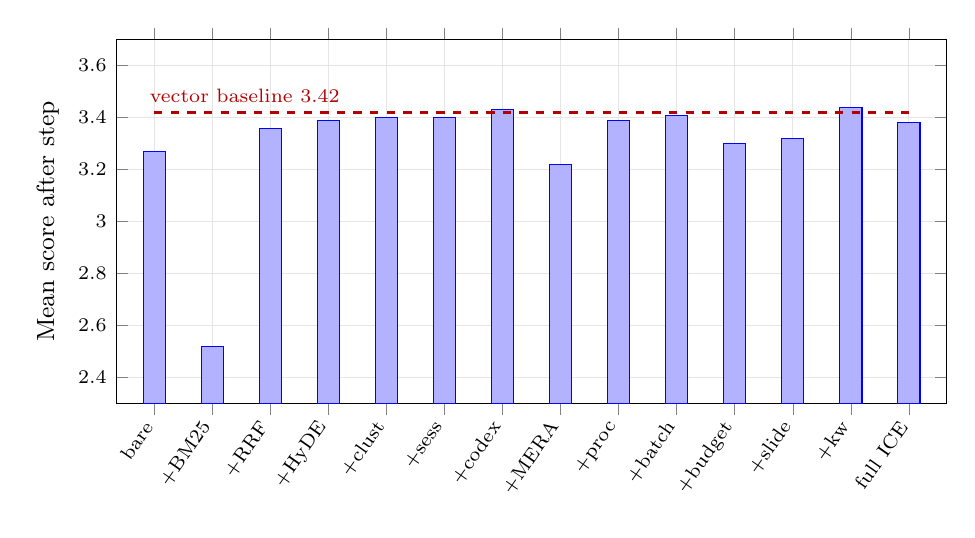
\begin{tikzpicture}
\begin{axis}[
    width=\columnwidth, height=6.2cm,
    ybar,
    bar width=8pt,
    ymin=2.3, ymax=3.7,
    ylabel={\small Mean score after step},
    ylabel near ticks,
    symbolic x coords={bare,+BM25,+RRF,+HyDE,+clust,+sess,+codex,+MERA,+proc,+batch,+budget,+slide,+kw,full ICE},
    xtick=data,
    x tick label style={rotate=55, anchor=east, font=\scriptsize},
    ytick={2.4,2.6,2.8,3.0,3.2,3.4,3.6},
    tick label style={font=\scriptsize},
    enlarge x limits=0.05,
    grid=major, grid style={gray!20},
    every axis plot/.append style={fill=blue!55!black, draw=blue!30!black},
]
\addplot coordinates {
 (bare,3.27) (+BM25,2.52) (+RRF,3.36) (+HyDE,3.39) (+clust,3.40)
 (+sess,3.40) (+codex,3.43) (+MERA,3.22) (+proc,3.39) (+batch,3.41)
 (+budget,3.30) (+slide,3.32) (+kw,3.44) (full ICE,3.38) };
\draw[dashed, red!70!black, thick] (axis cs:bare,3.42) -- (axis cs:full ICE,3.42)
  node[pos=0.12, above, font=\scriptsize, red!70!black] {vector baseline 3.42};
\end{axis}
\end{tikzpicture}
\caption{Feature ablation buildup (Dataset B, 67 probes, Experiment 3). Each bar is the cumulative mean score after adding one feature to all previous ones. The only two movements that clear a paired bootstrap CI are the $+$BM25 drop ($-0.74$) and the $+$RRF recovery ($+0.82$); all other step deltas are within noise, and several toggled features were non-functional at the snapshot (Section~\ref{sec:limitations}). The dashed line marks the single-leg vector baseline (3.42), which is not a step in the buildup; the full build finishes level with it.}
\label{fig:ablation-waterfall}
\end{figure}

\subsection{Comparative Summary}

Across the four experiments, the story is not ``ICE is always better''---it is ``ICE is more resilient and more efficient, and its advantage grows with conversation difficulty.'' Experiment 1 showed ICE could be worse than the baseline; Experiment 2 showed it can match quality with 32\% fewer fragments; the ICE-Dev stress test showed it can survive where the baseline collapses; the ablation showed that fusion rescues unfused multi-signal retrieval and---read together with a fidelity audit---that several components (procedural, RAG, batch summaries, HyDE) were never actually exercised and the Codex was under-weighted. The narrative is one of progressive, and ultimately self-correcting, understanding rather than single-result triumph.

%======================================================================
\section{Discussion}
\label{sec:discussion}

\subsection{What We Learned About Conversational Memory}

Memory is not just retrieval---it is \emph{curation}. ICE's advantage comes not from retrieving more (it retrieves less) but from retrieving better. The token budget, RRF fusion, and keyword boost are the mechanisms that measurably filter noise in our ablation; decay, cluster scoping, and session diversification are designed to the same end but were neutral on the single dataset we could ablate. A memory system that remembers everything is a memory system that remembers nothing useful. The fragment--score correlation is the cleanest empirical statement of this principle: for ICE, more fragments correlate positively with quality ($r = +0.19$); for the vector baseline, more fragments correlate negatively with quality ($r = -0.02$). Same metric, opposite sign.

\subsection{What the Ablation Can and Cannot Establish}

The buildup ablation cleanly establishes two things: that adding an unfused lexical leg is harmful, and that rank fusion recovers it. It cannot adjudicate the value of most of the features it toggles, because several were disabled, dead, or under-weighted at the snapshot (Section~\ref{sec:limitations})---a flat delta from a component that never ran is uninformative, not a domain-specific null. The one design lever the ablation does implicate is the token budget: its fill-to-cap policy over-injects on long conversations, which points not at ``more retrieval is bad'' but at the need for a marginal-relevance stopping rule. Beyond that, the honest reading is that the load-bearing mechanisms in this study were the unglamorous ones---fusion, the budget, and post-fusion curation---while the ambitious stores await a build in which they actually function. The classification-driven leg weighting, which conditions retrieval on inferred intent, remains the least-explored lever and the most likely source of future gains.

\subsection{How Do the Findings Generalise?}

The token-budget finding (ICE-Dev stress test) should generalise to any system that injects retrieved context into a fixed-context-window model. The RRF finding (ablation) should generalise to any multi-leg retrieval system. The methodological finding---that a component must be verified genuinely live before a null can be attributed to it---should generalise to any multi-component system evaluated by ablation. The fragment--score correlation finding is, we suspect, universal: a system whose fragments correlate negatively with answer quality is, in a deep sense, a system that does not know what it is doing.

%======================================================================
\section{Limitations}
\label{sec:limitations}

We are deliberately specific about what this study does and does not show. Several of these limitations directly motivate the future work of Section~\ref{sec:future-work}.

\subsection{Single-User Evaluation}
All benchmark conversations were authored by a single user. While the selected conversations span creative writing, technical planning, academic planning, and long-horizon worldbuilding, they still reflect the habits, vocabulary, and interaction style of one individual. The results therefore demonstrate effectiveness for a diverse set of conversation \emph{types} rather than for a diverse \emph{population of users}. Repetition of this evaluation across multiple users is a prerequisite for generalising the findings beyond the current study.

\subsection{Synthetic Longitudinal Reconstruction and Missing Reinforcement Loops}
The evaluation reconstructs conversation history by replaying existing conversations and periodically probing the resulting memory state. This allows controlled experimentation over hundreds or thousands of turns, but cannot fully replicate the feedback loops that occur during live usage. In real deployments, retrieval events continuously influence future memory states through reinforcement, decay adjustment, bookmarking, procedural extraction, and user behaviour; during evaluation, many of these interactions are absent because future turns already exist and cannot be influenced by retrieved outputs.

More specifically, ICE includes retrieval-strengthening mechanisms that increase the \texttt{access\_count} and partially restore the \texttt{decay\_score} of frequently accessed memories, while allowing unused memories to decay. During evaluation, retrieval reinforcement is driven almost entirely by benchmark probes rather than by natural user interaction. In a real conversation, a user might ask about a character's motivations every few sessions, reinforcing that memory repeatedly; in the evaluation, the memory receives reinforcement only when a probe explicitly targets it. Important concepts that would normally be revisited repeatedly during a live conversation therefore receive less reinforcement than they would in production usage, creating a more difficult retrieval environment than would be encountered during normal operation. Consequently, the benchmark likely \emph{underestimates} the benefits of reinforcement-driven memory maturation. The positive longitudinal curves observed in Experiment 2 are promising, but are likely a lower bound on real-world performance improvement.

\subsection{Routing Bias and Classifier Conservatism}
Between Experiment 1 and Experiment 2, the classifier was retrained with a substantially improved embedding backbone (Qwen3-Embedding-0.6B replacing MiniLM), which reduced gating failures from 22 to 2. However, a second change was also introduced: a conservative routing override applied \emph{after} classification. Queries classified as \texttt{Zero\_Shot} were automatically re-routed to \texttt{Long\_Term\_Memory} when confidence fell below a threshold, or when the conversation exceeded a certain turn count (the ``long-conversation LTM bias'').

One concrete failure mode motivated part of this override: a \textbf{public-entity trap}, in which the classifier learned to associate well-known proper nouns with \texttt{Zero\_Shot} (the model already ``knows'' who or what they are), even when the query was clearly scoped to the user's own conversation about that entity. A question referencing a famous, widely-known character name from Dataset A's fan-fiction work, for instance, was liable to be classified as requiring no retrieval at all---because the classifier had learned that the entity itself is public knowledge, not that the \emph{conversation} about it is the user's own long-running creative project. This was patched with a hard override forcing \texttt{Long\_Term\_Memory} for any conversation-scoped query, which is effective but crude: it does not distinguish between a public entity discussed in a genuinely stateless way and a public entity that is the subject of extensive private, user-specific elaboration. A more principled fix would require the classifier to condition on conversation history rather than the query text alone---which the context-aware classification path (Section~\ref{sec:architecture}) partially addresses, but not completely.

This override is a deliberate safety net: false negatives (failing to retrieve when memory is needed) are fatal, while false positives (retrieving when not strictly needed) are merely expensive. The empirical evidence from Experiment 1 supported this design---gating failures caused complete answer failures, whereas unnecessary retrieval only added modest context overhead. However, the override introduces a fundamental limitation: the system is no longer purely intent-aware in the way the architecture claims. ICE frequently forces retrieval even when the classifier predicts zero-shot, because the heuristic overrides the classifier's judgment. The system is therefore ``safe'' rather than ``smart''---it errs on the side of retrieval to avoid catastrophic forgetting, at the cost of occasionally injecting irrelevant context. The true strength of the classifier is thus masked by the override; we cannot claim that ICE's intent-gating is purely driven by the MLP, because the rule-based override is actively compensating for classifier uncertainty. A more principled approach would treat the classifier's confidence as a prior and combine it with a conversation-length prior via Bayesian inference, rather than applying a hard threshold.

\subsection{Codex Extraction Reliability}
The Codex subsystem is the most architecturally ambitious component of ICE and, in the current implementation, also the most fragile. Its marginal contribution in Experiment 2 (only 3.3\% of retrieved fragments, $+0.03$ in the ablation) does not reflect the subsystem's theoretical ceiling, but rather the cumulative effect of several simultaneous engineering handicaps.

\textbf{The chunking paradox.} Current extraction uses 6{,}000-token chunks with a 200-token overlap, chosen to avoid splitting sentences and to preserve broad narrative context. However, a 4B-parameter model does not possess the effective reasoning capacity to process 6{,}000 tokens simultaneously; beyond 1{,}000--1{,}500 tokens, attention becomes diluted, losing track of entities mentioned in the middle of the chunk while disproportionately weighting the beginning and end. This causes two failure modes: (1)~\emph{entity dropping}, where entities introduced mid-passage are never extracted; and (2)~\emph{relationship hallucination}, where the model confuses the subject and object of distant clauses, outputting syntactically valid but semantically meaningless triplets (e.g., \texttt{fastapi uses fastapi}). The optimal chunk size for reasoning with a 4B model is closer to 512--800 tokens, which was not used in the current evaluation.

\textbf{Weak confidence and strength signals.} Edges carry a \texttt{confidence}
flag in \{pending, active\} and a numeric \texttt{strength} that decays over time,
but both are under-utilised in retrieval. The Codex traversal follows any edge
with \texttt{valid\_until IS NULL}, regardless of confidence or strength, and the
only effect of \texttt{confidence == 'active'} is a coarse 1.5$\times$ score
boost at the fragment level. There is no reinforcement loop that strengthens
edges on retrieval, so frequently referenced facts do not rise in the ranking,
and traversal treats weak or decayed edges as equally important as strong ones.
Edge strength and confidence are therefore almost-inert signals that contribute
little to retrieval quality.

\textbf{Semantic versus lexical matching.} Codex retrieval is exact-match (canonical name or aliases) plus vector fuzzy matching over the \texttt{context\_payload} embedding, not the entity name itself. If a user establishes an entity ``The Obsidian Citadel'' and later asks ``where is the main fortress located?'', the entity resolution step has no lexical or embedded anchor for ``fortress'' to match against---even though a human reader immediately understands the reference. This is a fundamental limitation of entity-centric retrieval in free-form conversation: it assumes users consistently refer to entities by canonical names or close aliases, which is empirically false in natural dialogue.

\textbf{Implications.} The marginal contribution of Codex should be read as a floor, not a ceiling. That it produced any positive contribution despite oversized extraction chunks, a single-fragment retrieval representation, and no retrieval-time reinforcement suggests that a properly implemented Codex could become one of the strongest components in the architecture. The negative result for MERA ($-0.21$) is similarly contextual: MERA activates only when entity extraction finds no entities, so it is a downstream indicator of extraction gaps rather than an independent subsystem evaluation.

\subsection{Non-Functional and Disabled Components at the Evaluation Snapshot}
An honest fidelity audit of the evaluated build (tag \texttt{v2-paper-eval}) found that much of the retrieval machinery the architecture describes was not contributing. Of the six legs, \textbf{three returned nothing.} The \emph{procedural} and \emph{RAG} legs bound the query embedding as a plain array rather than a typed pgvector value, so under the deployed database driver every call raised a type error, rolled back, and returned an empty list (the procedural intent gate hid the failure); RAG was additionally gated off on these datasets and its store was empty. The \emph{batch-summary} leg was correctly implemented but its store was empty as well, because no turn in the replay decayed far enough to be batched. The \emph{Codex} leg was live but contributed only 3.3\% of fragments---an under-weighting of its content, not an entity-detection failure: NER loaded its trained model (${\sim}95\%$ recall), and the real handicaps were oversized extraction chunks, the single-fragment retrieval representation, and an inert confidence signal (detailed in the Codex subsection above). Separately, the \emph{HyDE} query-rewrite was commented out in the evaluated build. This is corroborated within the reported data: procedural, RAG, and batch summaries account for 0\% of injected fragments in Experiment~2 (Section~\ref{sec:exp2}); the two episodic legs supply 62.3\% and Codex 3.3\% (the remainder being unattributable), and the ablation's disabled or inactive steps move the score only within noise.

Two consequences follow, and we state them plainly. First, the reported results---the quality tie, the 32\% fragment reduction, and the context-overflow survival---were produced, in effect, by \emph{two working retrieval legs (BM25 and decay-weighted vector) plus a 3.3\% Codex contribution and a token budget}. If anything this \emph{sharpens} the central thesis: the system matched a strong baseline while most of its elaborate machinery was inactive, which is the strongest possible evidence that curation, not the number of stores, is what carries a memory system. Second, and crucially, \textbf{a non-functional component is not a measured null.} We make no claim that the knowledge graph, procedural memory, document store, or HyDE are unhelpful; we claim only that these results \emph{did not depend on them}. The binds and the HyDE path are fixed post-snapshot, and the true contribution of the repaired components is deferred to the FINAL re-evaluation (Section~\ref{sec:future-work}).

\subsection{Mixture-of-Experts Routing: Hardcoded, Untrained, and Latency-Bounded}
The MoE-vs-generalist comparison shows negligible differences (global $\Delta = +0.01$ for ICE, $-0.02$ for vector). The implemented router has three deficiencies that together explain this. First, routing is based on hardcoded topic/intent mappings rather than learned or empirical model-performance data; there is no signal that a model tagged \texttt{Software\_\&\_Tech} actually outperforms a generalist on software questions. Second, the router ignores classifier confidence---a \texttt{max\_confidence} of 0.55 is treated identically to 0.95. Third, it ignores context-reliance labels, routing self-contained \texttt{Zero\_Shot} queries identically to context-heavy \texttt{Long\_Term\_Memory} queries. An operational cost compounds these: when the router selects an unloaded model, Ollama unloads the current model and loads the new one (5--15~s), and ICE has no control over this process. The MoE infrastructure is therefore both conceptually underdeveloped and operationally costly.

\subsection{KV-Cache Optimisation: Designed but Largely Ineffective in Practice}
The Prompt Assembler uses stable-prefix ordering to maximise KV-cache reuse. In practice, cache hits are rare: the recent-turn window changes on every request (invalidating the prefix from that point on), the retrieved-context block changes on most queries, MoE model swaps wipe the cache entirely, and Ollama's cache is ephemeral and session-bound. The only reliably cacheable segments---the system message and persistent slots---account for roughly 10--15\% of the prompt. Stable-prefix ordering is the correct \emph{design}, but the practical benefit is limited by factors outside ICE's control.

\subsection{Judge Model Limitations and the Experiment 3 Audit Gap}
Evaluation relied primarily on an automated judge (\texttt{mattbucci/gemma-4-12B-AWQ}). During analysis, multiple cases were identified where correct, true information was incorrectly flagged as hallucinated because it was absent from the \emph{condensed} ground-truth summary rather than from the conversation itself---a systematic over-harshness that affected all four evaluated conditions equally, not a bias against any one system. To correct this, every hallucination flag across all 1{,}211 Experiment 2 probes was individually audited against the source conversation and corrected where the flagged detail was verifiably true; flags on genuine fabrications were left in place, and no credit was given for speculative or unverifiable additions. This is label correction, not score substitution---the judge's own criteria were applied more carefully, not replaced with human opinion. Experiment 3 (the ablation) was \emph{not} audited this way: because it evaluated fifteen closely related variants under identical conditions, manual adjustments would have risked introducing subjective bias across comparisons that are meant to isolate a single architectural change at a time. Its absolute hallucination values (e.g., the 41.4\% ICE-Dev rate) should therefore be interpreted cautiously as potentially inflated by the same automated-judge false positives described above; the \emph{relative} differences between conditions remain valid, but the absolute numbers should not be compared directly to Experiment 2's audited values.

\subsection{Hallucination Rates and the ICE-Dev Paradox}
ICE exhibits higher hallucination on Dataset C (41.4\% generalist) than globally (20.2\%), despite achieving its highest absolute score there (4.33). The apparent contradiction is resolved by the denominator: the vector baseline failed on 94.2\% of ICE-Dev probes (no answer), yielding a 0\% hallucination rate \emph{by definition}. ICE, because it survives these probes, generates answers and therefore has opportunities to hallucinate. The rate reflects the difficulty of the task, not a failure mode unique to ICE.

\subsection{Further Scope Limitations}
\textbf{Probe generation bias.} Most probes were generated through a constrained LLM-assisted pipeline; generated questions may differ from the more context-dependent, anaphoric, pragmatically ambiguous questions real users ask. This is partially mitigated by 72 manually authored probes carried over from earlier experiments, but the benchmark remains weighted toward automatically generated probes. \textbf{Domain coverage.} The four domains omit collaborative software development, multi-user conversations, customer support, multilingual dialogue, and workplace communication, where multi-party dynamics or formal structures may change performance. \textbf{Cross-conversation retrieval.} ICE contains infrastructure for cross-conversation search, but every probe targets a single conversation; within-conversation memory is demonstrated, cross-conversation aggregation is not yet validated. \textbf{Decay horizon.} The longest simulated horizon is 93 days; year-scale stability, saturation, and the eventual convergence of decay dynamics remain open. \textbf{Hardware-constrained ablation.} All experiments ran on a single 24GB RTX 5090. The Experiment 3 ablation used Qwen3-14B-AWQ rather than the 26B generalist to fit 15 conditions $\times$ 67 probes in a reasonable time; relative deltas hold, but absolute scores are systematically lower than Experiment 2's, and the system has not been evaluated on enterprise-grade (80GB+) hardware. \textbf{No comparison with commercial systems.} ChatGPT's memory and Claude's project features cannot be run locally with controlled retrieval; the vector-RAG baseline is the strongest fair comparison constructible on identical hardware.

%======================================================================
\section{Future Work}
\label{sec:future-work}

The limitations above defined a research program that we have since substantially implemented in the released system, post-dating the \texttt{v2-paper-eval} snapshot these results reflect. We describe it both as the agenda the evaluation motivated and as a record of what already exists to be re-measured; none of it affects the numbers reported above, and its rigorous longitudinal re-evaluation is the FINAL study described at the end.

\subsection{Self-Correcting Codex Extraction}
The passive triplet collector has been replaced by a reconciliation-based pipeline: deterministic NER grounding produces a confirmed entity list, relationship mapping is constrained to those entities (removing hallucinations such as \texttt{fastapi uses fastapi}), and every proposed triplet is checked against the graph so that a contradiction opens a bounded reconciliation loop---antonym reversals resolved deterministically, ambiguous supersessions escalated to the review queue rather than blind-written. A code-aware layer emits deterministic \texttt{imports}/\texttt{calls}/\texttt{inherits} edges directly from source. This targets the Codex fragility of Section~\ref{sec:limitations}; the remaining work is chunk-size tuning and the confidence-calibrated edge storage the retrieval scorer needs.

\subsection{Agentic Background Maintenance}
The fixed background workers are now orchestrated by a Memory Maintenance Agent---a lightweight LLM given a tool set (\texttt{merge\_conflicting\_entities}, \texttt{reconcile\_graph\_state}, \texttt{flag\_for\_review}, \texttt{run\_cluster\_consolidation}) that reconciles graph state during idle GPU time and decides autonomously whether to extract, merge, or escalate, with the review queue preserved as the human-in-the-loop safety net. The scheduler beneath it replaced the Celery/Redis worker fleet with an in-process maintenance runtime triggered by session-end, overdue, and work-unit events.

\subsection{Density-Robust Retrieval}
The ICE-Dev collapse motivated retrieval at the 512-token chunk level plus a raw/summary/abstract representation hierarchy, so a single 8{,}000-token turn can no longer dominate the budget, and a model-aware budget now derives its ceiling from the routed model's context window. The open piece is need-based (marginal-relevance) stopping---the principled fix for the ablation's fill-to-cap dynamic-budget regression, replacing the turn-bracket growth formulas.

\subsection{Temporal, Cross-Conversation, and Coding Memory}
A temporal-retrieval layer now answers as-of, range, and evolution queries (``how did my design for X change over time'')---the axis no probe in this study exercised. A Project State Engine extends memory across a project's entire history---architecture clusters, decisions, git-commit facts, tasks---for a coding mode, and ICE now exposes itself as an MCP server for headless use. A conversation-import path ingests exported chat logs through the very replay pipeline used here for evaluation, reconstructing full episodic, graph, procedural, and cluster state rather than a searchable archive---directly attacking the vendor lock-in of cloud memory.

\subsection{Learned Routing, Continual Learning, and Transparency}
The still-open frontier: a learned MoE router conditioned on classifier confidence, context-reliance, and empirical per-model performance (replacing the hardcoded scorer this study found neutral); an opt-in continual-learning loop folding thumbs-up/down feedback into the weekly classifier fine-tune; and an explainability layer exposing per-fragment retrieval attribution and an editable Codex graph.

\subsection{FINAL: Re-Evaluation of the Repaired System}
The concrete next study re-runs the full protocol with confidence intervals computed from the first probe, pre-registered memory-deletion rules, a matched-prompt baseline (isolating retrieval from prompt assembly), a re-measurement of the components non-functional or disabled at this snapshot (procedural, RAG, batch summaries, HyDE), and a new temporal probe class scored on era-correctness and evolution narration---so the temporal and now-repaired components are measured rather than assumed.

%======================================================================
\section{Conclusion}
\label{sec:conclusion}

We have presented a local-first conversational memory system (ICE)---a multi-store architecture with intent-driven retrieval routing, a temporally-versioned knowledge graph, and a per-query dynamic token budget---and LSREP, a longitudinal evaluation protocol that measures not retrieval quality at a single instant but memory accumulation, retention, and belief revision across months of conversational history. Evaluated under LSREP, the system matches a strong vector-RAG baseline on answer quality while injecting 32\% fewer fragments, wins a substantially larger share of blind head-to-head comparisons, and survives a context-overflow stress test where the unbudgeted baseline collapses to a 94.2\% failure rate. A cumulative ablation shows that unfused multi-signal retrieval is harmful and that rank fusion is corrective. We have been deliberate that this is a first, honest measurement rather than a verdict: a fidelity audit found that several of the more ambitious stores were immature or inactive at the evaluated snapshot, so the demonstrated gains rest on curation, fusion, and the token budget, and the fuller architecture awaits the re-evaluation set out in Section~\ref{sec:future-work}.

As context windows grow, the temptation is to simply stuff more context in. Our results suggest the opposite: in long-horizon conversational AI, less-but-better context matches a firehose on raw quality while beating it on efficiency, head-to-head preference, and survival under density. The future of conversational memory is not bigger windows---it is smarter curation. ICE's architecture, with its classification-driven routing, RRF-based fusion, and per-query token budget, points toward a design philosophy where the memory system acts as a \emph{curator} rather than a \emph{firehose}. We hope this work contributes to that philosophy and that the released implementation, evaluation protocol, and ablation harness enable others to build on it.

%======================================================================
\section*{Broader Impact and Reproducibility}

The substantive limitations of this work are enumerated in full in Section~\ref{sec:limitations}: single-user evaluation, synthetic longitudinal reconstruction, classifier-override conservatism, Codex extraction fragility, three retrieval legs (procedural, RAG, batch summaries) non-functional and HyDE disabled at the evaluated snapshot, the neutrality of the MoE router, ineffective KV-caching in practice, the Experiment 3 audit gap, and constrained domain and hardware coverage. We add two further observations on reproducibility and ethics.

\textbf{Reproducibility.} The full source code, the evaluation harness, and the experimental configuration are released as part of this work. All reported results reflect the system as it existed at the evaluation-time snapshot, preserved in the repository as the git tag \texttt{v2-paper-eval} (the tag preserves the evaluated \emph{code}; companion artifacts written after the snapshot---this paper and the archived technical report---live on the repository's main branch); the implementation has continued to evolve since. All numbers reported in Section~\ref{sec:results} are derived from publicly shareable JSON reports; the raw judge-model outputs and the LSREP probe sets are not released because they contain personal conversational content. A distinction is worth stating plainly: the \emph{protocol} is fully reproducible, but the \emph{data} is not manufacturable. The four corpora are real conversations accumulated through genuine use over months to years---Dataset~B alone represents roughly a year of actual interaction---and their evaluation value derives precisely from that authenticity: the entity evolution, contradictions, superseded decisions, and long-range dependencies are organic, not planted. An equivalent corpus cannot be synthesised on demand, and this is a general property of longitudinal memory evaluation rather than a limitation specific to this study. Reproducing the evaluation therefore means bringing one's own long-form conversational history (most platforms support chat-log export, which the replay harness ingests); the protocol, harness, judge configuration, and metrics transfer unchanged to any such corpus.

\textbf{Ethical considerations.} All four evaluation datasets were created by the first author, who is the sole data subject. No third-party conversational data was used. The system stores the user's own data on the user's own hardware; no data leaves the local machine. The architecture includes a memory-slot system in which high-stakes steering slots (project context, user preferences, guidance) require explicit user approval before Reflection-proposed updates are applied, while low-stakes bookkeeping (pending items) is autonomous. This human-in-the-loop boundary is a deliberate design choice rather than a performance limitation.

\textbf{Societal implications.} ICE is deliberately local-first: memory lives on the user's own hardware and no conversational data leaves the machine, a privacy posture cloud-hosted memory cannot offer. By making persistent, structured memory viable on a single consumer GPU, the architecture also lowers the barrier to capable personal AI that does not depend on a metered cloud API---a modest step toward broadening who can run such systems. The same persistence is, however, dual-use: a system that faithfully models a user's evolving beliefs, preferences, and history could be turned toward profiling or manipulation as readily as toward assistance, especially if the memory store were moved off the user's control. We raise this not because the present work enables it---the system is single-user, local, inspectable, and fully exportable and deletable by construction---but because the very properties that make ICE benign (local storage, human-in-the-loop memory edits, user-controlled retention) are precisely the ones a harmful variant would strip away. We therefore regard keeping those user-sovereignty properties non-negotiable as part of the contribution, not incidental to it.

%======================================================================
\begin{thebibliography}{99}
\small

\bibitem[Packer et al.(2023)]{packer2023memgpt}
Charles Packer, Sarah Wooders, Kevin Lin, Vivian Fang, Shishir G. Patil, Ion Stoica, and Joseph E. Gonzalez. 2023. MemGPT: Towards LLMs as Operating Systems. \emph{arXiv preprint}. Available at \url{https://www.semanticscholar.org/paper/MemGPT%3A-Towards-LLMs-as-Operating-Systems-Packer-Fang/908dad62c0e43d80e3e3cb3c0402f7c71c70499c}.

\bibitem[Chhikara et al.(2025)]{chhikara2025mem0}
Prateek Chhikara, Abhinav Khant, et al. 2025. Mem0: Building Production-Ready AI Agents with Scalable Long-Term Memory. \emph{arXiv preprint}, arXiv:2504.19413. Available at \url{https://arxiv.org/abs/2504.19413}.

\bibitem[Zhong et al.(2024)]{zhong2024memorybank}
Wanjun Zhong, Lianghong Guo, et al. 2024. MemoryBank: Enhancing Large Language Models with Long-Term Memory. \emph{Proceedings of the AAAI Conference on Artificial Intelligence}. Available at \url{https://ojs.aaai.org/index.php/AAAI/article/view/29946}.

\bibitem[Shi et al.(2024)]{shi2024scmoe}
Chufan Shi, Cheng Yang, et al. 2024. Unchosen Experts Can Contribute Too: Unleashing MoE Models' Power by Self-Contrast. \emph{arXiv preprint}, arXiv:2405.14507. Available at \url{https://arxiv.org/abs/2405.14507}.

\bibitem[Cai et al.(2024)]{cai2024scmoe}
Weilin Cai, Juyong Jiang, Le Qin, Junwei Cui, Sunghun Kim, and Jiayi Huang. 2024. Shortcut-connected Expert Parallelism for Accelerating Mixture-of-Experts. \emph{arXiv preprint}, arXiv:2404.05019. Available at \url{https://arxiv.org/html/2404.05019v3}.

\bibitem[Edge et al.(2024)]{edge2024graphrag}
Darren Edge et al. 2024. From Local to Global: A Graph RAG Approach to Query-Focused Summarization. \emph{Microsoft Research}. Available at \url{https://www.microsoft.com/en-us/research/publication/from-local-to-global-a-graph-rag-approach-to-query-focused-summarization/}.

\bibitem[Wang et al.(2023)]{wang2023kgp}
Yu Wang, Nedim Lipka, Ryan A. Rossi, Alexa Siu, Rui Zhang, and Tyler Derr. 2023. Knowledge Graph Prompting for Multi-Document Question Answering. \emph{arXiv preprint}, arXiv:2308.11730. Available at \url{https://arxiv.org/abs/2308.11730}.

\bibitem[Sun et al.(2024)]{sun2024tog}
Jiashuo Sun et al. 2024. Think-on-Graph: Deep and Responsible Reasoning of Large Language Model on Knowledge Graph. \emph{ICLR Proceedings}. Available at \url{https://proceedings.iclr.cc/paper_files/paper/2024/file/10a6bdcabbd5a3d36b760daa295f63c1-Paper-Conference.pdf}.

\bibitem[Lewis et al.(2020)]{lewis2020rag}
Patrick Lewis, Ethan Perez, Aleksandra Piktus, Fabio Petroni, Vladimir Karpukhin, Naman Goyal, Heinrich K\"uttler, Mike Lewis, Wen-tau Yih, Tim Rockt\"aschel, Sebastian Riedel, and Douwe Kiela. 2020. Retrieval-Augmented Generation for Knowledge-Intensive NLP Tasks. \emph{Advances in Neural Information Processing Systems 33 (NeurIPS 2020)}. Available at \url{https://proceedings.neurips.cc/paper_files/paper/2020}.

\bibitem[Guu et al.(2020)]{guu2020realm}
Kelvin Guu, Kenton Lee, Zora Tung, Panupong Pasupat, and Ming-Wei Chang. 2020. REALM: Retrieval-Augmented Language Model Pre-Training. \emph{Proceedings of the 37th International Conference on Machine Learning (ICML 2020)}, PMLR 119:3929--3938. Available at \url{https://proceedings.mlr.press/v119/guu20a.html}.

\bibitem[Izacard and Grave(2021)]{izacard2021fid}
Gautier Izacard and Edouard Grave. 2021. Leveraging Passage Retrieval with Generative Models for Open Domain Question Answering. \emph{ACL Anthology}, EACL. Available at \url{https://aclanthology.org/2021.eacl-main.74/}.

\bibitem[Shi et al.(2024)]{shi2024replug}
Weijia Shi, Sewon Min, Michihiro Yasunaga, Minjoon Seo, Rich James, Mike Lewis, Luke Zettlemoyer, and Wen-tau Yih. 2024. REPLUG: Retrieval-Augmented Black-Box Language Models. \emph{Proceedings of NAACL 2024}, pages 8371--8384. Available at \url{https://aclanthology.org/2024.naacl-long.463/}.

\bibitem[Yan et al.(2024)]{yan2024crag}
Shi-Qi Yan, Jia-Chen Gu, Yun Zhu, and Zhen-Hua Ling. 2024. Corrective Retrieval Augmented Generation. \emph{arXiv preprint}, arXiv:2401.15884. Available at \url{https://arxiv.org/abs/2401.15884}.

\bibitem[Robertson and Zaragoza(2009)]{robertson2009bm25}
Stephen Robertson and Hugo Zaragoza. 2009. The Probabilistic Relevance Framework: BM25 and Beyond. \emph{Foundations and Trends in Information Retrieval}. Available at \url{https://www.staff.city.ac.uk/~sbrp622/papers/foundations_bm25_review.pdf}.

\bibitem[Cormack et al.(2009)]{cormack2009rrf}
Gordon V. Cormack, Charles L. A. Clarke, and Stefan B\"uttcher. 2009. Reciprocal Rank Fusion Outperforms Condorcet and Individual Rank Learning Methods. \emph{SIGIR '09: Proceedings of the 32nd International ACM SIGIR Conference on Research and Development in Information Retrieval}, pages 758--759. Available at \url{https://doi.org/10.1145/1571941.1572114}.

\bibitem[Gao et al.(2023)]{gao2023hyde}
Luyu Gao, Xueguang Ma, Jimmy Lin, and Jamie Callan. 2023. Precise Zero-Shot Dense Retrieval without Relevance Labels. \emph{Proceedings of the 61st Annual Meeting of the Association for Computational Linguistics (ACL 2023)}, pages 1762--1777. Available at \url{https://aclanthology.org/2023.acl-long.99/}.

\end{thebibliography}

%======================================================================
\appendix
\section{Implementation Reference}
\label{app:implementation}

This appendix collects the operational detail that supports the architecture of Section~\ref{sec:architecture} but is not required to follow the paper's main argument. It is reproduced here for readers reimplementing the system.

\subsection{Background Worker Cluster}
\label{app:workers}

\begin{table}[htbp]
\centering
\small
\caption{Background workers. The cluster is self-maintaining---no operator intervention is required for the memory lifecycle.}
\label{tab:workers}
\begin{tabular}{@{}L{3.2cm}L{2.6cm}L{7cm}@{}}
\toprule
\textbf{Worker} & \textbf{Trigger} & \textbf{Function} \\
\midrule
Post-Flight Evaluator & every turn & lossless detection, summary, dispatch extractors \\
Codex Extractor      & lossless turns  & triplet extraction, handle\_triplet writes \\
Procedural Extractor  & every turn      & pattern detection, reinforcement or insertion \\
Episodic Decay        & 1.5 h           & access-weighted decay, archive at 0.1, cold-store at 0.05 \\
Codex Decay           & 1.5 h           & edge strength decay, demote at strength $<$ 0.3 \\
Procedural Decay      & 1.5 h           & boolean deactivation after 180 d if $<$ 3 reinforcements \\
Clustering            & 30 min          & assign unassigned turns to clusters, merge similar \\
Reflection            & 2 h             & session synthesis, pattern crystallisation, slot proposals \\
Batch Summariser      & 2 h             & 50-turn batches, preservation-prompt summaries \\
Sentinel Monitor      & 30 min          & declarative rules: threshold, absence, etc. \\
Fine-Tune             & weekly (Mon 04:00 UTC) & retrain classifier head on curated labels \\
Compaction            & manual          & snapshot entities with $\geq$100 uncompacted events \\
Drop Zone             & filesystem      & ingest .txt/.jsonl/.md into RAG store \\
Codex Inject Watcher  & filesystem      & ingest .yaml/.json into Codex with manual confidence \\
\bottomrule
\end{tabular}
\end{table}

All GPU-touching workers gate on \texttt{is\_gpu\_busy()} (a 20\%-utilisation threshold polled via \texttt{nvidia-smi}) and, in shared mode, additionally on \texttt{is\_user\_active()} (the Redis key \texttt{ice:last\_chat\_completed} within a 10-second idle window). Retry countdowns are fixed: 15~s post-flight, 30~s extractors, 60~s decay/sentinel/compaction/reflection, 120~s batch-summariser/cluster-merge. All workers are idempotent through an \texttt{idempotency\_key} UNIQUE column, turning Celery's at-least-once delivery into effectively-once side effects.

\subsection{Operational Infrastructure}

The system is a single FastAPI service (\texttt{/v1/chat/completions} for the OpenAI-compatible endpoint plus routers for memory slots, user control, and model registry), backed by PostgreSQL with the pgvector extension (one \texttt{Vector(384)} column per vector table because the embedder is shared), and a Celery worker fleet over Redis. The configuration system is a Pydantic \texttt{Settings} reading from \texttt{.env}. The active inference path loads \texttt{ice\_classifier\_v3\_qwen\_ft3.pt}; classifier fine-tuning writes a timestamped file but does not auto-promote it, so production promotion requires a manual file swap. SSE event types (\texttt{classified}, \texttt{retrieval}, \texttt{context\_ready}, \texttt{generating}, \texttt{degraded}) drive the observability panel and downstream monitoring.

A complete technical reference, including the full training pipeline for the classifier and NER models, the controlled relation vocabulary in its entirety, the complete worker implementation, GPU resource management, idempotency architecture, and operational infrastructure, is available in the technical report archived in the repository (\texttt{docs/ICE\_Architecture[real\_v2].md}).

\end{document}
